% T14c of the Transport Papers series (companion to T14). Number confirmed by Leon (2026-11-20: T14c, to be uploaded
\documentclass[11pt]{article}
\usepackage[margin=1.1in]{geometry}
\usepackage{amsmath,amssymb,amsthm,mathtools}
\usepackage{booktabs}
\usepackage{array}
\usepackage[hyphens]{url}
\usepackage[dvipsnames]{xcolor}
\usepackage{tikz}
\usetikzlibrary{arrows.meta,calc,decorations.pathreplacing}
\usepackage[colorlinks=true,linkcolor=MidnightBlue,citecolor=MidnightBlue,urlcolor=MidnightBlue]{hyperref}

\newtheorem{theorem}{Theorem}[section]
\newtheorem{proposition}[theorem]{Proposition}
\newtheorem{lemma}[theorem]{Lemma}
\newtheorem{corollary}[theorem]{Corollary}
\theoremstyle{definition}
\newtheorem{definition}[theorem]{Definition}
\newtheorem{remark}[theorem]{Remark}
\newtheorem{fact}[theorem]{Fact}
\newtheorem{premise}[theorem]{Premise}
\newtheorem{observation}[theorem]{Observation}
\newtheorem{computation}[theorem]{Computation}

\newcommand{\Cl}{\mathrm{Cl}}
\newcommand{\R}{\mathbb{R}}
\newcommand{\C}{\mathbb{C}}
\newcommand{\HH}{\mathbb{H}}
\newcommand{\F}{\mathbb{F}}
\newcommand{\rev}[1]{\widetilde{#1}}
\newcommand{\ip}[1]{\langle #1 \rangle}
\newcommand{\Neff}{N_{\mathrm{eff}}}
\newcommand{\su}{\mathfrak{su}}
\newcommand{\so}{\mathfrak{so}}
\newcommand{\uu}{\mathfrak{u}}
\newcommand{\sll}{\mathfrak{sl}}
\newcommand{\gl}{\mathfrak{gl}}
\newcommand{\file}[1]{\texttt{#1}}
\newcommand{\hatV}{\widehat{V}}
\newcommand{\hf}{\hat{f}}
\newcommand{\Mat}{\mathrm{M}}
\newcommand{\pstep}[1]{\par\smallskip\noindent\textit{#1.}\enspace}
\newcommand{\pitem}[1]{\par\smallskip\noindent\textit{#1}\enspace}
\setlength{\emergencystretch}{1.5em}

\title{\bfseries The Matter in the Dark Towers\\[4pt]
  \large\itshape Companion note to T14: what each tower is made of, built by the Standard-Model paper's construction in geometric algebra}
\author{Leon Butler\\ \normalsize\href{mailto:lbutler.math@gmail.com}{\texttt{lbutler.math@gmail.com}}\\ \normalsize ORCID: \href{https://orcid.org/0009-0006-4449-5617}{0009-0006-4449-5617}}
\date{Version 1.0, November 2026 \textperiodcentered{} Transport Papers, T14c}

\begin{document}
\maketitle

\begin{abstract}
\normalsize
The dark-matter paper T14 fixes how much matter each of five dark towers holds, not what that matter is. This note builds it with the Standard-Model paper's construction. A constituent is an element of the spin-irreducible even ideal of the tower's conformal algebra, and its scalars are the commutant of the spin action there. We prove that this field is the division algebra of the next residue: the reals in the three-dimensional towers, the complex numbers in this tower and the mirror, the quaternions in the five-dimensional towers. One identity of the reversion pairing then says where mass begins (two constituents in three and four dimensions, one in five); the momentum-preserving mixings are the field's unitary groups; and, under the series' identification premise and one transposition rule, the gauge algebras follow. The mirror carries the Standard Model again. Both three-dimensional towers carry the abelian $\so(2) \oplus \so(2)$: two copies of single-flavour electrodynamics in $2+1$ dimensions. Both five-dimensional towers carry $\uu(3)$, dark colour and one abelian charge, with vector-like quarks, leptons and a neutral singlet; with an external imaginary unit both would carry the Standard-Model algebra instead. The towers of each odd dimension differ only in discrete structure. Three consequences follow. Neither the unit-ball rule's premise E nor T14's particle model has a mechanism in any odd tower. A cold mirror is an unstated exception to T14's indifference premise. No configuration of the towers as built passes the cluster, radiation and mirror bounds together. The algebraic results are verified in exact arithmetic.
\end{abstract}

\medskip
\noindent\textbf{MSC 2020.} Primary 15A66, 83F05; Secondary 81V25, 85A40, 81T13.\\
\textbf{Keywords.} geometric algebra; Clifford algebra periodicity; spinor ideals; dark matter; hidden sectors; mirror matter; parity anomaly; Kaluza-Klein radiation.

\newpage
\textbf{Authorship and disclosure. }The founding idea of the series is the author's: that division by zero in a Clifford algebra should be read not as a prohibition but as a transport into a higher-dimensional algebra, and that the transported division need not be accompanied by an inverse operation. The direction of investigation and the critical review of the results are likewise the author's. The mathematical development and the drafting of the text were carried out in extended collaboration with Claude Fable 5 (Anthropic), an AI system. The papers of the series are deposited in the Transport Papers community on Zenodo, \url{https://zenodo.org/communities/transport-papers}.

\newpage
\tableofcontents
\newpage

%=====================================================================================
\section{Introduction}\label{sec:intro}

The dark-matter paper T14 \cite{ButlerT14} derives eight parallel towers, one per residue $r = p - q \bmod 8$ of the real Clifford algebras, and finds that six can hold matter: this one ($r = 6$, signature $(1,3)$), its mirror ($r = 2$, $(3,1)$), two three-dimensional towers ($r = 1, 7$) and two five-dimensional towers ($r = 3, 5$). The towers touch only through the one shared metric. By its unit-ball rule the five dark towers hold, relative to our baryons, the shares $1$, $4/3$, $4/3$, $8/(3\pi)$ and $8/(3\pi)$, whose sum $(11\pi + 16)/(3\pi) = 5.364$ is the observed ratio of dark to visible matter. T14 proves the mirror a copy of this tower; for the four odd towers it says how much matter each holds and leaves open what that matter is.

This note answers that question by doing in each tower what the Standard-Model paper T12 \cite{ButlerT12} does in ours. T12's chain is: a constituent; the number of constituents at which mass begins; the mixings that preserve total momentum; the automorphisms of the smallest massive composite, identified with the gauge algebra; the content and its charges; then, with imported physics, hadrons, atoms and a stable relic. Every link is transposed here, and where the transposition meets an obstacle the resolution is taken from the way our tower resolves the same obstacle.

Everything is written in geometric algebra. A constituent is an element of a minimal left ideal of an even Clifford algebra; its momentum is the vector part of $\psi e_{t} \rev{\psi}$; its field of scalars is the corner algebra $f \Cl^{0} f$ with the adjoint $x^{\dagger} = e_{t}\rev{x}e_{t}^{-1}$. The mass laws are identities of the reversion pairing $\rev{\psi}_{1}\psi_{2}$.

\subsection*{Prior art}

The real Clifford algebras, their periodicity and their spinor modules are classical (Cartan, Chevalley \cite{Chevalley1954}, Lounesto \cite{Lounesto2001}); the even-subalgebra isomorphisms $\Cl^{0}(p,q) \cong \Cl(p,q-1)$ and $\Cl^{0}(p,q) \cong \Cl^{0}(q,p)$ are standard \cite{Porteous1995, Lounesto2001}, and the division algebra of each even algebra can be read off the periodicity table. The spacetime-algebra current $j = \psi\gamma_{0}\rev{\psi}$ and its square $j^{2} = |\psi\rev{\psi}|^{2}$ are Hestenes's \cite{Hestenes1966, DoranLasenby2003}. Mirror matter and its cosmology have a long literature \cite{FootMirror2004, RouxCline2020}; the parity anomaly and topologically massive gauge fields in $2+1$ dimensions are Redlich's and Deser, Jackiw and Templeton's \cite{Redlich1984, DJT1982}; Polyakov confinement \cite{Polyakov1977}; five-dimensional gauge theory, its Chern-Simons terms and its strong-coupling scale are standard \cite{IMS1997, CLP2000}. The identification of a gauge algebra with the automorphisms of the minimal massive composite is T12's, and its global form and content are classical structure theory once that identification is made.

\subsection*{Contribution}

\begin{enumerate}
\item The constituent's field in tower $r$ is the division algebra of residue $r + 1$, at the conformal and the tower level alike (Theorem \ref{thm:fields}, a corollary of the periodicity table): $\R$, $\C$, $\HH$ as the causal tower's dimension runs three, four, five. It is not the type T14 assigns by residue, which is the commutant of a different module (Remark \ref{rem:T14types}).
\item One identity of the reversion pairing gives where mass begins: at two constituents in three and four dimensions, where the pairing is alternating, and at one in five, where it is not (Theorem \ref{thm:onset}). The momentum-preserving mixings are $O(n)$, $U(n)$, $Sp(n)$ (Theorem \ref{thm:ladder}).
\item The third ladder pair of the five-dimensional towers needs a complex unit. At $r = 3$ the algebra supplies one, and every other quaternionic unit fails to commute with the pair structure; at $r = 5$ the units form a sphere (Theorem \ref{thm:unit}).
\item Under T12's identification premise and one transposition rule (Premise \ref{prem:U}): $\so(2) \oplus \so(2)$ in both three-dimensional towers, $\uu(3)$ in both five-dimensional towers ($\su(2) \oplus \su(3) \oplus \uu(1)$ in both if the pair unit is external), the Standard Model in the mirror (Theorem \ref{thm:algebras} and, for the mirror, T14's copy theorem), with the content of Propositions \ref{prop:content3} and \ref{prop:content5}.
\item The towers of each odd dimension hold the same kind of matter (Corollary \ref{cor:samekind}); the classical isomorphism of the mirror's even algebras with this tower's is made explicit as a real map, which reverses the conformal pseudoscalar (Theorem \ref{thm:mirror}).
\item The physics: the matter of each tower in halos (Section \ref{sec:matter}); neither T14's premise E nor its particle model has a mechanism in the odd towers, whose quanta are elementary or unconfined with bare masses, not the confined composites T14's Section 8 describes (Observation \ref{prop:R1}); a cold mirror is an exception to P2 (Proposition \ref{prop:P2}); and the towers as built against the data (Observation \ref{obs:data}).
\end{enumerate}

Table \ref{tab:summary} and Figure \ref{fig:clock} collect the result.

\begin{table}[ht]\centering\small\setlength{\tabcolsep}{4pt}
\begin{tabular}{@{}llllll@{}}
\toprule
$r$ & tower & field & gauge algebra & elementary matter & in halos \\
\midrule
$6$ & $(1,3)$, ours & $\C$ & $\su(3) \oplus \su(2) \oplus \uu(1)$ & quarks, leptons & atoms, stars \\
$2$ & $(3,1)$, mirror & $\C$ & the same & a copy & dissipative gas \\
$1$ & $(2,1)$, sheets & $\R$ & $\so(2) \oplus \so(2)$ & cells $A$, $B$ & collisionless in one phase \\
$7$ & $(1,2)$, sheets & $\R$ & $\so(2) \oplus \so(2)$ & cells $A$, $B$ & collisionless in one phase \\
$3$ & $(4,1)$ & $\HH$ & $\uu(3)$\,$^{*}$ & $U, D, E, N$, vector-like & free fermions \\
$5$ & $(1,4)$ & $\HH$ & $\uu(3)$\,$^{*}$ & $U, D, E, N$, vector-like & free fermions \\
$0$ & $(2,2)$ & $\R$ & $\sll(2,\R) \oplus \sll(3,\R) \oplus \gl(1,\R)$ & none (no stable vacuum) & none \\
$4$ & $(4,0)$, $(0,4)$ & $\HH$ & (no time) & none & none \\
\bottomrule
\end{tabular}
\caption{The eight towers' matter. Fields: Theorem \ref{thm:fields}. Gauge algebras: Theorem \ref{thm:algebras}, under H2 and Premise \ref{prem:U}; $^{*}$with an external pair unit, $\su(2) \oplus \su(3) \oplus \uu(1)$ in both (Remark \ref{rem:branches}); $r = 0$: Remark \ref{rem:kleinian}. Content: Propositions \ref{prop:content3}, \ref{prop:content5}. In halos: Section \ref{sec:matter}.}
\label{tab:summary}
\end{table}

\begin{figure}[ht]
\centering
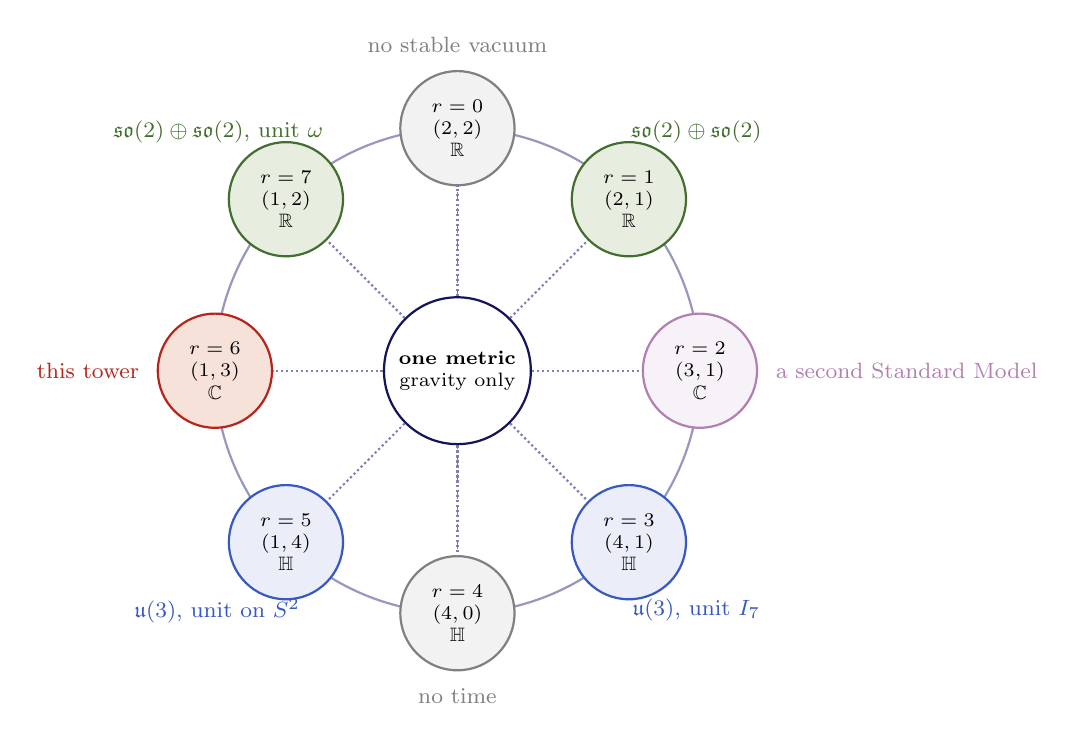
\begin{tikzpicture}[scale=1.12, >=stealth]
\draw[MidnightBlue!45, thick] (0,0) circle (2.75);
\draw[gray, dashed] (0,3.35) -- (0,-3.35);
\foreach \r/\lab/\col/\out in {
  0/{$r=0$\\$(2,2)$\\$\R$}/gray/{no stable vacuum},
  1/{$r=1$\\$(2,1)$\\$\R$}/OliveGreen!80!black/{$\so(2)\oplus\so(2)$},
  2/{$r=2$\\$(3,1)$\\$\C$}/Plum!80!black/{a second Standard Model},
  3/{$r=3$\\$(4,1)$\\$\HH$}/RoyalBlue!85!black/{$\uu(3)$, unit $I_{7}$},
  4/{$r=4$\\$(4,0)$\\$\HH$}/gray/{no time},
  5/{$r=5$\\$(1,4)$\\$\HH$}/RoyalBlue!85!black/{$\uu(3)$, unit on $S^{2}$},
  6/{$r=6$\\$(1,3)$\\$\C$}/BrickRed/{this tower},
  7/{$r=7$\\$(1,2)$\\$\R$}/OliveGreen!80!black/{$\so(2)\oplus\so(2)$, unit $\omega$}}{
  \node[circle, draw=\col, thick, fill=\col!10, minimum size=1.45cm,
        font=\scriptsize, align=center] (n\r) at ({90-45*\r}:2.75) {\lab};
  \node[\col, font=\footnotesize, anchor={270-45*\r}, align=center] at ({90-45*\r}:3.5) {\out};
  \draw[MidnightBlue!55, densely dotted, thick] (0,0) -- (n\r);
}
\node[circle, draw=MidnightBlue!80!black, thick, fill=white, minimum size=1.6cm, font=\scriptsize, align=center] at (0,0) {\textbf{one metric}\\gravity only};
\end{tikzpicture}
\caption{The eight towers on the residue clock, each with its signature under T14's Premise P3, the field of its constituents (Theorem \ref{thm:fields}) and what it carries. Across the dashed axis $r \mapsto -r$ the pairs $\{2, 6\}$, $\{1, 7\}$, $\{3, 5\}$ are exchanged; within each pair the field and the gauge algebra agree, and only discrete structure differs (Corollary \ref{cor:samekind}). The towers interact only through the one metric at the centre.}
\label{fig:clock}
\end{figure}

%=====================================================================================
\section{Setting, imports and premises}\label{sec:setting}

Throughout, a tower is $V = \R^{p,q}$ with an orthonormal basis $\{e_{a}\}$, $Q(e_{a}) = e_{a}^{2} = \pm 1$, and $\Cl(V) = \Cl(p,q)$ its Clifford algebra, with even subalgebra $\Cl^{0}(V)$, reversion $x \mapsto \rev{x}$, grade involution $x \mapsto \hat{x}$ and grade projection $\ip{\cdot}_{k}$. In a causal signature ($\min(p,q) = 1$) the \emph{time direction} $e_{t}$ is the one basis vector of the minority sign, as in T14's convention \cite[Prop.~3.1]{ButlerT14}, and $Q(e_{t}) = \pm 1$ accordingly. The tower's conformal algebra is $\Cl(\hatV)$ with $\hatV = V \oplus \R^{1,1}$, that is $\Cl(p+1, q+1)$. The pseudoscalar of an algebra of dimension $n$ is $\omega = e_{1}e_{2}\cdots e_{n}$, central when $n$ is odd, with $Q(\omega) = (-1)^{n(n-1)/2}(-1)^{q}$.

The objects that the twistor paper T9 \cite{ButlerT9} and T12 describe in twistor language are, here, the even ideals of the conformal algebra and their elements; this note uses only the latter.

\begin{fact}[imported: the towers and their types]\label{fact:towers}
The residue $r = p - q \bmod 8$ is constant along each tower of $(1,1)$ ascents. Under T14's Premise P3 the representatives are $(1,3)$ at $r = 6$, $(3,1)$ at $r = 2$, $(2,1)$ and $(1,2)$ at $r = 1, 7$, $(4,1)$ and $(1,4)$ at $r = 3, 5$, $(2,2)$ at $r = 0$ and $(4,0)$ or $(0,4)$ at $r = 4$; $r = 0$ and $r = 4$ are sterile. The odd residues carry no orientation bit and therefore no asymmetry. The towers interact only through the one metric (exact superselection). Sources: In odd dimension the orientation flag has one family, so it grades nothing \cite[Prop.~3.9]{ButlerT14}. Sources: \cite[Prop.~3.1, Thm.~3.4, Prop.~3.9, Thm.~3.10, Prop.~4.1]{ButlerT14}, \cite[Thm.~3.6]{ButlerT3}.
\end{fact}

\begin{fact}[imported: Clifford structure]\label{fact:clifford}
(i) For $q \geq 1$, $\Cl^{0}(p,q) \cong \Cl(p,q-1)$, by $e_{a} \mapsto e_{a}e_{n}$ with $Q(e_{n}) = -1$; for $p \geq 1$, $\Cl^{0}(p,q) \cong \Cl(q, p-1)$. (ii) $\Cl(p,q)$ is a matrix algebra over $D \in \{\R, \C, \HH\}$, or a sum of two, with $D$ fixed by $p - q \bmod 8$: $\R$ at $0, 1, 2$; $\C$ at $3, 7$; $\HH$ at $4, 5, 6$. (iii) A minimal left ideal $Af$ of a simple or semisimple algebra $A$, $f$ a primitive idempotent, has commutant $\mathrm{End}_{A}(Af) \cong (fAf)^{\mathrm{op}}$, a division algebra (Schur), acting by right multiplication. Sources: \cite{Chevalley1954, Lounesto2001, LawsonMichelsohn1989}.
\end{fact}

\begin{fact}[imported: our tower's chain]\label{fact:chain}
In this tower: a single constituent has null momentum and two have the squared mass of T11's two-constituent formula \cite[Prop.~4.1]{ButlerT11}, \cite[Fact~2.1]{ButlerT12}; each constituent carries three ladder pairs \cite[Fact~2.2, Lem.~2.12]{ButlerT12}, the tower's rungs satisfying the canonical anticommutation relations \cite[Prop.~4.1]{ButlerT3}; the mixings of $n$ constituents preserving their total momentum and helicity form are $U(n)$ \cite[Prop.~3.1]{ButlerT12}; and the content, hypercharges, anomalies and Higgs representation are \cite[Thm.~4.1, Thm.~4.2, Prop.~5.3, Thm.~5.5, Prop.~9.22]{ButlerT12}.
\end{fact}

\begin{fact}[imported: the unit-ball rule]\label{fact:rule}
T14's unit-ball rule rests on two premises: E, one length $d$ common to every populated tower at which each holds the same mass per ball of radius $d$ of its own space, and R3, a three-dimensional tower's sheets stacked one $d$ apart and a five-dimensional tower's matter counted through one $d$ of its extra direction. Under E and R3 the shares are $1$, $2 \times 4/3$, $2 \times 8/(3\pi)$, with total $(11\pi + 16)/(3\pi)$ \cite[Prem.~7.2, Prem.~7.4, Prop.~7.6(i)]{ButlerT14}. T14's particle model, R1 (every quantum of every populated tower has the same mass) and R2 (one quantum per unit ball of each tower's own space, so a common Wigner-Seitz radius $d$), implies E and is not used by the rule \cite[Prem.~7.3, Prop.~7.6(ii)]{ButlerT14}; in it $d$ is this world's baryon spacing, $d_{b} \approx 0.98$ m, and the mass the nucleon's \cite[Rem.~7.9, Cor.~7.26]{ButlerT14}. E alone fixes neither. As fractions of the dark matter: mirror $18.6$ percent, each three-dimensional tower $24.9$, each five-dimensional tower $15.8$.
\end{fact}

\begin{fact}[imported: the cluster simulations]\label{fact:sims}
In the idealised Bullet-like merger runs of T14b \cite[Obs.~7.1, Table~3]{ButlerT14b}: (i) with only the mirror colliding ($18.6$ percent of the dark matter, as gas) the subcluster keeps a separate lensing peak on its galaxies and a mass-to-light change of $0.82$ against the observed $0.84 \pm 0.07$; (ii) with the mirror gas and one three-dimensional tower's share of colliding fluid ($43.5$ percent colliding) the subcluster dissolves, and with more it dissolves too; (iii) with the mirror collisionless and $24.9$ or $31.6$ percent of colliding fluid, the subcluster keeps a weaker peak but only $0.55$ or $0.44$ of its central mass: the colliding fluid alone costs about half of it. In (i) the subcluster's own mass is $0.57$ of the cold-dark-matter run's, a deficit T14b notes is larger than the $23$ percent bound on it; T14b takes the mass-to-light change, the quantity that bound is inferred from, as the test, and by that test the run is consistent, since mass and light leave together \cite[Obs.~7.1]{ButlerT14b}. No run lies between $18.6$ and $24.9$ percent colliding. The colliding components there are fluids.
\end{fact}

\begin{fact}[imported: gauge theory in three dimensions]\label{fact:threeD}
(i) A two-component fermion of unit charge shifts the Chern-Simons level of its $U(1)$ by $\tfrac{1}{2}\mathrm{sign}(m)$ (the parity anomaly) \cite{Redlich1984, NiemiSemenoff1983}. (ii) A Chern-Simons level $k \neq 0$ gives the photon the topological mass $e^{2}k/2\pi$, and then a compact $U(1)$ does not confine \cite{DJT1982, AHPS1989}. (iii) A compact $U(1)$ with Maxwell dynamics alone confines \cite{Polyakov1977}. (iv) Flux attachment shifts the spin of a charge $q$ by $q^{2}/2k$ \cite{Wilczek1982}.
\end{fact}

\begin{fact}[imported: gauge theory in five dimensions]\label{fact:fiveD}
Five-dimensional gauge theory is infrared free, with a strong-coupling scale set by $g_{5}^{2}$, and the abelian cubic Chern-Simons coefficient $\tfrac{1}{2}\sum \mathrm{sign}(m)\,q^{3}$ of a five-dimensional fermion content must be integral \cite{IMS1997, CLP2000}.
\end{fact}

\begin{fact}[imported: dark-plasma bounds]\label{fact:plasma}
Plasma-instability limits on the charge of a dark-matter plasma in cluster mergers are those of \cite{SSS2024, PIC2024}; whether such instabilities transfer bulk momentum in a merger is not established \cite{Lasenby2020}.
\end{fact}

\begin{fact}[imported: the mirror copy]\label{fact:mirrorcopy}
The mirror tower carries a copy of this tower's matter: the same gauge algebra $\su(2) \oplus \su(3) \oplus \uu(1)$, global form $S(U(2) \times U(3))$ and content \cite[Thm.~4.3]{ButlerT14}.
\end{fact}

Four statements are carried as premises. H1 and H2 are this paper's names for two of T12's ingredients used off dimension four; Hypothesis (S) is T12's; U is this paper's transposition rule.

\begin{premise}[H1: momentum]\label{prem:H1}
A constituent has a spinor part $\psi$ in the tower's spinor ideal $S$ (Definition \ref{def:ideals}), carried by a map $T \to S$ that intertwines the action of the tower's spin group, so that the field of $T$ acts on $S$ through it; its momentum is the vector part of $\psi e_{t}\rev{\psi}$. In dimension four this is T12's Fact 2.1 in the even algebra; in dimensions three and five it is a premise.
\end{premise}

\begin{premise}[H2: identification]\label{prem:H2}
The gauge algebra of a tower's matter is the automorphism algebra of its minimal massive hierarchy, constituent slots tensor pair slots, as T12's Theorem 4.1 identifies it in dimension four, at observation level \cite[Thm.~4.1, Prop.~4.3]{ButlerT12}.
\end{premise}

\begin{premise}[Hypothesis (S): slot statistics]\label{prem:S}
The constituent slots are fermionic modes on the same footing as the pairs, so that the composite's state space is the exterior algebra of slot and pair modes \cite[Sec.~5]{ButlerT12}. Used only where stated.
\end{premise}

\begin{premise}[U: transposition rule]\label{prem:U}
(U1) A constituent is an element of the spin-irreducible even ideal of the conformal algebra, as T12 defines this tower's, and its field is the commutant of the spin action on it. (U2) The hierarchy's first factor counts constituents at mass onset, and its slot group is the momentum-preserving group of that many constituents; the pair group is the group of mixings of the ladder pairs that preserves their canonical relations and the field's positive norm, the unitary group over the pairs' scalars ($\R$, or $\C$ where a complex unit builds the pairs), as T12 takes $U(m) \times U(k)$ \cite[Thm.~4.1]{ButlerT12}. The norm clause is part of the premise: no positive form on the pair space is derived here, and without it the group preserving the canonical relations is $GL(2,\R)$ (see after Theorem \ref{thm:algebras}). The compactness of every gauge group below rests on it. (U3) Every complex unit used to build a ladder pair is an element of the constituent's field that the real algebra supplies; no external imaginary unit is adjoined.
\end{premise}

\begin{remark}[why U]\label{rem:whyU}
(U1) and (U2) are how this tower does it: T12's constituent is one chirality half of the ascended spinor module, which is spin-irreducible \cite[Fact~2.2]{ButlerT12}; its $\C^{2}$ is two constituents and its $U(2)$ their momentum ladder; and T12 takes both factors' groups unitary. (U3) is this paper's rule, not T12's. T12 builds its pairs in the complexification of the conformal space \cite[Fact~2.2, Lem.~2.12]{ButlerT12}. In this tower the two readings coincide: the even algebra $\Cl^{0}(2,4) \cong \Mat_{4}(\C)$ \cite[Rem.~3.2]{ButlerT9} has centre spanned by $1$ and the pseudoscalar $I_{6}$, so the commutant of the spin action on the constituent ideal is $\mathrm{span}\{1, I_{6}\}$, and any complex unit commuting with it, the complexification's included, acts there as $\pm I_{6}$. The readings part only where the field is $\HH$, in the five-dimensional towers, and there they give different gauge algebras (Remark \ref{rem:branches}): U3 is a choice, made because the series works in the real algebra. A further rule, the commutant of the full Clifford module read on its irreducible module, reproduces this tower too, but would make the mirror's constituents real and contradict T14's copy theorem; U1 does not.
\end{remark}

%=====================================================================================
\section{Constituents, momentum and where mass begins}\label{sec:constituents}

\begin{definition}[ideals, fields, momentum]\label{def:ideals}
Let $\hf$ be a primitive idempotent of $\Cl^{0}(\hatV)$, and in a causal tower let $f = \tfrac{1}{2}(1 + e_{t}e_{a})$ for a space direction $e_{a}$, which is a primitive idempotent of $\Cl^{0}(V)$ in dimensions three to five (Theorem \ref{thm:fields}); in the sterile towers $f$ is any primitive idempotent of $\Cl^{0}(V)$. The \emph{constituent ideal} is $T = \Cl^{0}(\hatV)\hf$ and the \emph{spinor ideal} is $S = \Cl^{0}(V)f$. Their \emph{fields} are the commutants $\F(T) = \mathrm{End}_{\Cl^{0}(\hatV)}(T)$ and $\F(S) = \mathrm{End}_{\Cl^{0}(V)}(S)$, the latter realised as right multiplication by the corner algebra $f\Cl^{0}(V)f$. In a causal tower the \emph{adjoint} is $x^{\dagger} = e_{t}\rev{x}e_{t}^{-1}$, and the \emph{momentum} of $\psi \in S$ is
\[
j(\psi) \;=\; \ip{\psi e_{t} \rev{\psi}}_{1}.
\]
The total momentum of constituents $\psi_{1}, \ldots, \psi_{n}$ is $P = \sum_{i} j(\psi_{i})$, and its \emph{squared mass} is $m^{2} = Q(e_{t})\,Q(P)$.
\end{definition}

The commutant of the spin action is the commutant of the even algebra, since the bivectors generate $\Cl^{0}$ as an algebra; so U1's field and the field of this definition agree. The constructions are explicit: $e_{t}e_{a}$ squares to $+1$, and $\Cl^{0}(V)f$ has real dimension $2$, $4$, $8$ in dimensions three, four, five, which is minimal (Theorem \ref{thm:fields}); $\hf$ is a product of two or three commuting factors $\tfrac{1}{2}(1 + b)$ with $b$ an even blade of square $+1$. The script builds both by a search over commuting even blades (Part A).

\begin{theorem}[the constituent's field]\label{thm:fields}
In tower $r$ the fields $\F(T)$ and $\F(S)$ are isomorphic, each to the division algebra of residue $r + 1$:
\begin{center}\small
\begin{tabular}{@{}lccccccccc@{}}
\toprule
$r$ & $6$ & $2$ & $1$ & $7$ & $3$ & $5$ & $0$ & $4$ \\
tower & $(1,3)$ & $(3,1)$ & $(2,1)$ & $(1,2)$ & $(4,1)$ & $(1,4)$ & $(2,2)$ & $(4,0)$, $(0,4)$ \\
conformal & $(2,4)$ & $(4,2)$ & $(3,2)$ & $(2,3)$ & $(5,2)$ & $(2,5)$ & $(3,3)$ & $(5,1)$, $(1,5)$ \\
field & $\C$ & $\C$ & $\R$ & $\R$ & $\HH$ & $\HH$ & $\R$ & $\HH$ \\
$\dim_{\R} T$, $\dim_{\R} S$ & $8, 4$ & $8, 4$ & $4, 2$ & $4, 2$ & $16, 8$ & $16, 8$ & $4, 2$ & $8, 4$ \\
\bottomrule
\end{tabular}
\end{center}
In particular the field is not a function of the conformal pseudoscalar's square: $Q(\omega) = -1$ at $r = 7$ (field $\R$) and at $r = 3$ (field $\HH$).
\end{theorem}

\begin{proof}
\textit{The two even algebras.}\enspace By Fact \ref{fact:clifford}(i),
\begin{align*}
\Cl^{0}(\hatV) &= \Cl^{0}(p+1, q+1) \cong \Cl(p+1, q), \\
\Cl^{0}(V) &= \Cl^{0}(p, q) \cong \Cl(p, q-1),
\end{align*}
and both have residue $(p+1) - q = p - (q-1) = r + 1$. The one tower with $q = 0$ is $(4,0)$: there $\Cl^{0}(4,0) \cong \Cl(0,3)$, of residue $-3 \equiv 5 = r + 1$, and $(0,4)$ gives the same algebra.

\pstep{The commutant} By Fact \ref{fact:clifford}(ii) each algebra is a matrix algebra over the division algebra $D(r+1)$, or a sum of two copies of one, and by Fact \ref{fact:clifford}(iii) the commutant of a minimal left ideal is $D(r+1)$. Reading $D$ off for each tower:
\[
\begin{array}{c|cccccccc}
r & 6 & 2 & 1 & 7 & 3 & 5 & 0 & 4 \\
r + 1 & 7 & 3 & 2 & 0 & 4 & 6 & 1 & 5 \\ \hline
D(r+1) & \C & \C & \R & \R & \HH & \HH & \R & \HH
\end{array}
\]

\pstep{Checks} The script computes every commutant from scratch on exact matrix representations of the ideals and classifies it (checks A1, A2), with the dimensions (A3) and the pseudoscalars (A4, A5).
\end{proof}

\begin{remark}[T14's types are a different commutant]\label{rem:T14types}
T14's Theorem 3.4 assigns real type to $r = 1, 2$, complex type with an intrinsic $U(1)$ to $r = 3, 7$, and quaternionic type to $r = 4, 5, 6$ \cite[Thm.~3.4]{ButlerT14}. That is the commutant of the full Clifford algebra $\Cl(V)$ on its irreducible module; Theorem \ref{thm:fields} is the commutant of the spin action on the constituent ideal. Both are correct and they answer different questions. T14's intrinsic $U(1)$ at $r = 3$ and $r = 7$ is the central pseudoscalar, which reappears here as structure the tower carries beside its constituent field: at $r = 7$ as a unit joining two real constituents (Proposition \ref{prop:omega7}), at $r = 3$ as the unit $I_{7}$ inside the quaternions (Theorem \ref{thm:unit}).
\end{remark}

\begin{lemma}[the adjoint and the norm]\label{lem:norm}
In a causal tower:
\begin{enumerate}
\item[(i)] $e_{K}e_{K}^{\dagger} = Q(e_{t})^{|K|}$ for every basis blade $e_{K}$, so $e_{K}e_{K}^{\dagger} = 1$ on every even blade and, for even $x$, $\ip{xx^{\dagger}}_{0}$ is the sum of the squares of $x$'s coordinates;
\item[(ii)] $f^{\dagger} = f$, and for $x \in f\Cl^{0}(V)f$,
\[
x^{\dagger}x \;=\; xx^{\dagger} \;=\; N(x)\,f, \qquad N(x) = 2\ip{xx^{\dagger}}_{0} \geq 0,
\]
with $N(x) = 0$ only at $x = 0$;
\item[(iii)] for $\psi \in S$ and $x \in f\Cl^{0}(V)f$,
\[
j(\psi x) \;=\; N(x)\, j(\psi).
\]
\end{enumerate}
\end{lemma}

\begin{proof}
\textit{(i) The blades.}\enspace Every direction other than $e_{t}$ has square $-Q(e_{t})$. There are two cases.

If $t \notin K$, moving $e_{t}$ through the $|K|$ vectors of $\rev{e_{K}}$ costs one sign each, and a blade times its reverse is the product of its squares:
\[
e_{K}^{\dagger} = e_{t}\rev{e_{K}}e_{t}^{-1} = (-1)^{|K|}\rev{e_{K}}, \qquad e_{K}\rev{e_{K}} = \bigl(-Q(e_{t})\bigr)^{|K|},
\]
so $e_{K}e_{K}^{\dagger} = (-1)^{|K|}\bigl(-Q(e_{t})\bigr)^{|K|} = Q(e_{t})^{|K|}$.

If $e_{K} = e_{t}e_{K'}$, then $\rev{e_{K}} = \rev{e_{K'}}e_{t}$, and
\begin{align*}
e_{K}^{\dagger} &= e_{t}\rev{e_{K'}} = (-1)^{|K'|}\,\rev{e_{K'}}\,e_{t}, \\
e_{K}e_{K}^{\dagger} &= (-1)^{|K'|}\,e_{t}\bigl(e_{K'}\rev{e_{K'}}\bigr)e_{t} = (-1)^{|K'|}\bigl(-Q(e_{t})\bigr)^{|K'|}\,Q(e_{t}) = Q(e_{t})^{|K|}.
\end{align*}
For $K \neq L$, $e_{K}e_{L}^{\dagger}$ is a multiple of $e_{K \triangle L}$, which has no scalar part. Hence for even $x = \sum_{K}x_{K}e_{K}$,
\[
\ip{xx^{\dagger}}_{0} \;=\; \sum_{K,L}x_{K}x_{L}\,\ip{e_{K}e_{L}^{\dagger}}_{0} \;=\; \sum_{K}x_{K}^{2} \qquad \text{(check B0)}.
\]

\pstep{(ii) The corner and its conjugation} With $f = \tfrac{1}{2}(1 + e_{t}e_{a})$ and $\rev{(e_{t}e_{a})} = e_{a}e_{t}$,
\[
f^{\dagger} = \tfrac{1}{2}\bigl(1 + e_{t}\,e_{a}e_{t}\,e_{t}^{-1}\bigr) = \tfrac{1}{2}(1 + e_{t}e_{a}) = f.
\]
The corner $\F = f\Cl^{0}f$ is a division algebra $\R$, $\C$ or $\HH$ with unit $f$ (Fact \ref{fact:clifford}(iii)). It is closed under $\dagger$, since $(fxf)^{\dagger} = fx^{\dagger}f$, and $\dagger$ is an anti-involution of it with $\ip{xx^{\dagger}}_{0} > 0$ for $x \neq 0$ by (i).

The standard conjugation is the only anti-involution with that positivity. Every other candidate has an element with $xx^{\dagger} = -f$, whose scalar part is $-\tfrac{1}{2}$:
\begin{itemize}
\item on $\C$ the other candidate is the identity, and a unit square root $x$ of $-f$ gives $xx^{\dagger} = xx = -f$;
\item on $\HH$ every other anti-involution is $x \mapsto u\bar{x}u^{-1}$ for a unit imaginary $u$, and a unit imaginary $v$ anticommuting with $u$ gives $v\,u\bar{v}u^{-1} = v^{2} = -f$.
\end{itemize}
So $\dagger$ is the standard conjugation, and
\[
x^{\dagger}x \;=\; xx^{\dagger} \;=\; N(x)\,f
\]
with $N$ the standard norm; the script verifies this as a polynomial identity in $x$'s coordinates (check B1). Taking scalar parts, with $\ip{f}_{0} = \tfrac{1}{2}$,
\[
\ip{xx^{\dagger}}_{0} \;=\; N(x)\,\ip{f}_{0} \;=\; \tfrac{1}{2}\,N(x),
\]
which is positive definite by (i), since $x$ is even (B3).

\pstep{(iii) The norm law} By the definition of the adjoint, $e_{t}\rev{x} = x^{\dagger}e_{t}$, and $\psi f = \psi$ for $\psi \in S$. So
\begin{align*}
\psi x\,e_{t}\,\rev{(\psi x)} &= \psi\,\bigl(x e_{t}\rev{x}\bigr)\,\rev{\psi} \\
&= \psi\,\bigl(xx^{\dagger}\bigr)\,e_{t}\rev{\psi} \\
&= N(x)\,\psi f\,e_{t}\rev{\psi} \\
&= N(x)\,\psi e_{t}\rev{\psi},
\end{align*}
and the grade-one part is $j(\psi x) = N(x)\,j(\psi)$ (B2).
\end{proof}

\begin{theorem}[where mass begins]\label{thm:onset}
Let $\psi, \psi_{1}, \psi_{2} \in S$ in a causal tower of dimension $n$.
\begin{enumerate}
\item[(i)] For $n = 3$ and $n = 4$ the reversion pairing is alternating, $\rev{\psi}\psi = 0$, every single constituent's momentum is null, and
\[
m^{2}\bigl(j(\psi_{1}) + j(\psi_{2})\bigr) \;=\; 2\,\ip{xx^{\dagger}}_{0}, \qquad x = \rev{\psi}_{1}\psi_{2}.
\]
Mass begins at two constituents; it vanishes exactly when $\rev{\psi}_{1}\psi_{2} = 0$.
\item[(ii)] For $n = 5$ the reversion pairing is not alternating, and
\[
m^{2}\bigl(j(\psi)\bigr) \;=\; \tfrac{1}{2}\,\ip{xx^{\dagger}}_{0}, \qquad x = \rev{\psi}\psi,
\]
which vanishes on a nonzero proper cone in $S$. Mass begins at one constituent.
\end{enumerate}
In every causal tower the total momentum of any number of constituents is timelike or null, never spacelike.
\end{theorem}

\begin{proof}
\textit{The pairing as a sandwich.}\enspace Write $\psi = \phi f$ with $\phi \in \Cl^{0}(V)$ and $f = \tfrac{1}{2}(1 + b)$, $b$ a bivector of square $+1$. Then $\rev{b} = -b$, so $\rev{f} = 1 - f$ and
\[
\rev{\psi}\psi \;=\; (1 - f)\;\rev{\phi}\phi\;f.
\]
The element $\rev{\phi}\phi$ is even and reversion-invariant, so it has grades $0$ and $4$ only:
\[
\rev{\phi}\phi = s + F, \qquad s = \ip{\rev{\phi}\phi}_{0}, \quad F = \ip{\rev{\phi}\phi}_{4}.
\]
Since $(1 - f)f = 0$, every part of $\rev{\phi}\phi$ that commutes with $b$ drops out of the sandwich:
\[
(1 - f)\,c\,f \;=\; c\,(1 - f)f \;=\; 0 \qquad \text{whenever } cb = bc.
\]

\pstep{Dimensions three and four} In dimension three $F = 0$. In dimension four $F = uI$ is a multiple of the pseudoscalar, which commutes with every even element and in particular with $b$. In both cases all of $\rev{\phi}\phi$ commutes with $b$, so $\rev{\psi}\psi = 0$. This is the alternation in (i).

\pstep{Dimension five} Here $F$ is a general four-vector, which need not commute with $b$, and $(1 - f)\,F f \neq 0$ for suitable $\phi$, so the pairing is not alternating.

\pstep{The mass laws} The two displayed laws are identities between polynomials of degree four in the coordinates of $\psi_{1}, \psi_{2}$ (respectively $\psi$) on a basis of $S$. The script verifies them as polynomial identities over $\mathbb{Q}$, not on samples, in all six causal towers (checks B4, B5), together with the nullity of $j(\psi)$ in dimensions three and four (B4); it exhibits a nonzero $\psi$ with $\rev{\psi}\psi = 0$ in each five-dimensional tower (B6). The right-hand sides are nonnegative by Lemma \ref{lem:norm}(i), so each single momentum (and in dimensions three and four each pair sum) is timelike or null.

\pstep{Any number of constituents} For every $\psi \in S$,
\begin{align*}
Q(e_{t})\,\bigl(j(\psi)\cdot e_{t}\bigr) &= Q(e_{t})\,\ip{\psi e_{t}\rev{\psi}\,e_{t}}_{0} \\
&= \ip{\psi\,e_{t}\rev{\psi}e_{t}^{-1}}_{0} \\
&= \ip{\psi\psi^{\dagger}}_{0} \;\geq\; 0 \qquad \text{(B7)}.
\end{align*}
So every constituent's momentum is causal and lies in the same closed half-space bounded by $e_{t}^{\perp}$, hence in the same half of the causal cone, and that half is closed under addition.
\end{proof}

\begin{remark}[the four-dimensional case is T11's formula]\label{rem:T11}
In this tower $x = \rev{\psi}_{1}\psi_{2}$ lies in the two-dimensional space $(1-f)\Cl^{0}f$, a copy of $\C$, and Theorem \ref{thm:onset}(i) is T11's two-constituent mass formula \cite[Prop.~4.1]{ButlerT11} written in the even algebra, the pairing $x$ playing the role of the bracket. In five dimensions the law is the classical Fierz identity of a single Dirac spinor, which in geometric algebra says that the four-vector part of $\rev{\phi}\phi$ survives the idempotent.
\end{remark}

\begin{theorem}[the ladder]\label{thm:ladder}
Let $\F = f\Cl^{0}(V)f$ act on $S$ on the right and on $S^{n}$ by $\psi'_{i} = \sum_{k}\psi_{k}U_{ki}$ for $U \in M_{n}(\F)$. Then $U$ preserves the total momentum of every $n$-tuple if and only if $UU^{\dagger} = 1$, where $(U^{\dagger})_{ik} = (U_{ki})^{\dagger}$. Momentum alone suffices here, where T12 also uses helicity \cite[Prop.~3.1]{ButlerT12}, because the mixings considered are $\F$-linear. The momentum-preserving group is $O(n)$, $U(n)$ or $Sp(n)$ as $\F = \R$, $\C$, $\HH$: $O(n)$ in the three-dimensional towers, $U(n)$ in this tower and the mirror, $Sp(n)$ in the five-dimensional towers.
\end{theorem}

\begin{proof}
\textit{Unitary mixings preserve the momentum.}\enspace Using $e_{t}\rev{y} = y^{\dagger}e_{t}$ on each entry of $U$,
\begin{align*}
\sum_{i}\psi'_{i}e_{t}\rev{\psi'_{i}} &= \sum_{i}\sum_{k,l}\psi_{k}U_{ki}\,e_{t}\,\rev{U_{li}}\,\rev{\psi_{l}} \\
&= \sum_{k,l}\psi_{k}\Bigl(\sum_{i}U_{ki}U_{li}^{\dagger}\Bigr)e_{t}\rev{\psi_{l}}.
\end{align*}
If $UU^{\dagger} = 1$, that is $\sum_{i}U_{ki}U_{li}^{\dagger} = \delta_{kl}f$, the right-hand side is $\sum_{k}\psi_{k}e_{t}\rev{\psi_{k}}$.

\pstep{Only unitary mixings do} Take $\psi_{k} = \psi a_{k}$ for one $\psi \in S$ with $j(\psi) \neq 0$ and a row $a = (a_{k}) \in \F^{n}$. Then $\psi'_{i} = \psi\,(aU)_{i}$, and Lemma \ref{lem:norm}(iii) gives the total momenta before and after as
\[
P = \Bigl(\sum_{k}N(a_{k})\Bigr)\,j(\psi), \qquad P' = \Bigl(\sum_{i}N\bigl((aU)_{i}\bigr)\Bigr)\,j(\psi).
\]
Their equality for every $a$ says that $U$ preserves the positive definite form $\sum_{k}N(a_{k})$ on $\F^{n}$, whose polarisation is the standard $\F$-Hermitian form; so $UU^{\dagger} = 1$.

\pstep{The groups} The isometry groups of the standard forms over $\R$, $\C$, $\HH$ are $O(n)$, $U(n)$, $Sp(n)$, and Theorem \ref{thm:fields} assigns the fields. The script checks an $\F$-unitary mixing in every causal tower as a polynomial identity (C1) and exhibits a non-unitary mixing that changes the total momentum (C2).
\end{proof}

%=====================================================================================
\section{The ladder pairs and the complex unit}\label{sec:pairs}

A \emph{ladder pair} is a pair $w, v$ of null vectors of the conformal space, $Q(w) = Q(v) = 0$, or of vectors dressed by a complex unit with $w^{2} = v^{2} = 0$, such that $wv + vw = 1$: the canonical anticommutation relations, one fermionic mode per pair \cite[Prop.~4.1]{ButlerT3}. Pairs built from real hyperbolic planes of $\hatV$ need no unit; their number is the real Witt index $\min(p,q) + 1$. The constituent's pair count is the complex Witt index $\lfloor (n+2)/2 \rfloor$ (T12's Lemma 2.12 in even dimension \cite[Lem.~2.12]{ButlerT12}; in odd dimension the same bound, with one generator left over).

\begin{proposition}[the pairs]\label{prop:pairs}
\begin{enumerate}
\item[(i)] In the three-dimensional towers the real and complex Witt indices of $\hatV$ are both $2$: two real ladder pairs, and no unit is needed (check D1).
\item[(ii)] In this tower, the mirror and the five-dimensional towers the real Witt index is $2$ and the complex one $3$: the third pair needs a complex unit. In this tower and the mirror the field is $\C$ and the unit is fixed up to sign (Remark \ref{rem:whyU}).
\end{enumerate}
\end{proposition}

\begin{proof}
In a causal tower $\min(p,q) = 1$, and $\hatV$ has signature $(p+1, q+1)$. Its Witt indices are
\[
\text{real: } \min(p+1, q+1) = 2, \qquad
\text{complex: } \Bigl\lfloor \frac{\dim\hatV}{2} \Bigr\rfloor =
\begin{cases} 2, & \dim\hatV = 5, \\ 3, & \dim\hatV = 6, 7. \end{cases}
\]
Check D1 builds the two real pairs of $\Cl(3,2)$ and $\Cl(2,3)$ on their modules and verifies the relations.
\end{proof}

\begin{theorem}[the third pair's unit in five dimensions]\label{thm:unit}
Work on the sixteen-dimensional irreducible module of the conformal algebra, which is the constituent ideal $T$ as a module of the spin group, with spin commutant $\HH$ (Theorem \ref{thm:fields}).
\begin{enumerate}
\item[(i)] ($r = 3$) The pseudoscalar $I_{7}$ of $\Cl(5,2)$ lies in $\HH$, squares to $-1$ and commutes with every vector. With it the third pair $\tfrac{1}{2}(e_{a} \pm I_{7}e_{b})$ joins two real pairs to give three pairs obeying the canonical relations, and their bilinears $I_{7}(v_{i}w_{i} - \tfrac{1}{2})$, $v_{i}w_{k} - v_{k}w_{i}$, $I_{7}(v_{i}w_{k} + v_{k}w_{i})$ span a Lie algebra $\uu(3)$ whose centraliser in $\HH$ is $\mathrm{span}\{1, I_{7}\}$.
\item[(ii)] ($r = 3$) Every unit $J \in \HH$ anticommuting with $I_{7}$ anticommutes with every vector, so it acts as the grade involution: it fixes the real pairs up to sign and sends $w_{3}$ to $-\bar{w}_{3}$, exchanging the third pair's creator and annihilator; $\uu(3)$ and $J$ generate a Lie algebra of dimension $30$, not the commuting sum $\su(2) \oplus \uu(3)$ of dimension $12$.
\item[(iii)] ($r = 5$) No element of $\HH$ outside $\R$ commutes with all of $\HH$, and $\omega$ squares to $+1$: the algebra supplies no canonical unit. Every unit $u \in \HH$ commutes with the vectors and builds a third pair, $w_{3} = \tfrac{1}{2}(e_{a} + ue_{b})$, $v_{3} = -\tfrac{1}{2}(e_{a} - ue_{b})$ with $Q(e_{a}) = Q(e_{b}) = -1$; the resulting $\uu(3)_{u}$ has centraliser $\mathrm{span}\{1, u\}$ in $\HH$, and a second unit anticommuting with $u$ generates dimension $30$ with it. Any two units are conjugate in $\HH$: $(1 - u'u)\,u = u'(1 - u'u)$ for $u' \neq -u$, and $u' = -u$ is reached by conjugation with any unit anticommuting with $u$. The choices form the sphere $Sp(1)/U(1) = S^{2}$.
\end{enumerate}
\end{theorem}

\begin{proof}
\textit{(i) The unit $I_{7}$.}\enspace $I_{7}$ is central in $\Cl(5,2)$ (odd dimension) with $Q(I_{7}) = -1$ (Section \ref{sec:setting}). Central elements commute with the spin action, so $I_{7} \in \HH$. Take $Q(e_{a}) = Q(e_{b}) = +1$ and
\[
w = \tfrac{1}{2}(e_{a} + I_{7}e_{b}), \qquad \bar{w} = \tfrac{1}{2}(e_{a} - I_{7}e_{b}).
\]
Since $I_{7}$ commutes with vectors and $e_{a}e_{b} = -e_{b}e_{a}$,
\begin{align*}
w^{2} &= \tfrac{1}{4}\bigl(Q(e_{a}) + I_{7}^{2}\,Q(e_{b})\bigr) = \tfrac{1}{4}(1 - 1) = 0, \\
w\bar{w} + \bar{w}w &= \tfrac{1}{2}\bigl(Q(e_{a}) - I_{7}^{2}\,Q(e_{b})\bigr) = \tfrac{1}{2}(1 + 1) = 1.
\end{align*}
The cross relations with the real pairs hold because distinct basis vectors anticommute and $I_{7}$ commutes with them (D3). Closure and the centraliser are computed (D4, D5).

\pstep{(ii) A unit anticommuting with $I_{7}$} $J$ commutes with the even algebra (it lies in the spin commutant) and anticommutes with $I_{7}$. Every vector factors as $e = (eI_{7}^{-1})\,I_{7}$ with $eI_{7}^{-1}$ even, so
\[
JeJ^{-1} \;=\; (eI_{7}^{-1})\,\bigl(JI_{7}J^{-1}\bigr) \;=\; (eI_{7}^{-1})(-I_{7}) \;=\; -e \qquad \text{(D6)}.
\]
Hence $J(I_{7}e_{b})J^{-1} = I_{7}e_{b}$ and
\[
Jw_{3}J^{-1} \;=\; -\tfrac{1}{2}(e_{a} - I_{7}e_{b}) \;=\; -\bar{w}_{3},
\]
and the closure has dimension $30$ (D7).

\pstep{(iii) The residue-five tower} The centre of $\HH$ is $\R$ and $Q(\omega) = +1$ (A4), so the algebra names no unit. The spin and Clifford commutants coincide on this module (D8), so every unit $u \in \HH$ commutes with the vectors. With $Q(e_{a}) = Q(e_{b}) = -1$ and $u^{2} = -1$,
\[
w_{3}v_{3} + v_{3}w_{3} \;=\; -\tfrac{1}{2}\bigl(Q(e_{a}) - u^{2}\,Q(e_{b})\bigr) \;=\; -\tfrac{1}{2}(-1 - 1) \;=\; 1 \qquad \text{(D9 to D11)}.
\]
For the conjugacy, with $u^{2} = u'^{2} = -1$,
\begin{align*}
(1 - u'u)\,u &= u - u'u^{2} = u + u', \\
u'\,(1 - u'u) &= u' - u'^{2}u = u' + u,
\end{align*}
so the two sides agree, and $1 - u'u = 0$ only at $u' = -u$ (D12).
\end{proof}

\begin{remark}[the two readings of the unit]\label{rem:units}
Theorem \ref{thm:unit} is where the two five-dimensional towers part. At $r = 3$ the unit that builds the pairs is fixed by the algebra, and the quaternionic unit group of a single constituent, which preserves its momentum (Theorem \ref{thm:ladder}), does not preserve the pair structure. At $r = 5$ every choice of unit is equivalent, and each choice cuts the quaternionic group to the circle it generates. Under U3 both towers therefore build their pairs with one complex unit; they differ in whether the algebra names it. With an external unit, which commutes with the whole quaternionic group, the group survives in both towers alike (Remark \ref{rem:branches}).
\end{remark}

%=====================================================================================
\section{The gauge algebras}\label{sec:algebras}

\begin{theorem}[the gauge algebras]\label{thm:algebras}
Under H2 and Premise \ref{prem:U}:
\begin{enumerate}
\item[(i)] (Three-dimensional towers, $r = 1, 7$.) Mass begins at two real constituents and each carries two real pairs, so the minimal massive hierarchy is $\R^{2} \otimes \R^{2}$. Its automorphisms $A \otimes B$ with $A, B \in O(2)$ form $(O(2) \times O(2))/\mathbb{Z}_{2}$, the kernel being $\{(1,1), (-1,-1)\}$; the gauge algebra is $\so(2) \oplus \so(2)$, abelian, of dimension $2$, and the identity component of the group is $U(1)_{+} \times U(1)_{-}$.
\item[(ii)] (Five-dimensional towers, $r = 3, 5$.) Mass begins at one constituent and its three pairs are complex with the unit of Theorem \ref{thm:unit}, so the hierarchy is $\C^{1} \otimes \C^{3}$. Its automorphisms form $(U(1) \times U(3))/U(1) \cong U(3)$; the gauge algebra is $\uu(3) = \su(3) \oplus \uu(1)$, of dimension $9$.
\end{enumerate}
\end{theorem}

In the mirror the algebra and global form are this tower's, $\su(2) \oplus \su(3) \oplus \uu(1)$ and $S(U(2) \times U(3))$: that is T14's copy theorem (Fact \ref{fact:mirrorcopy}), which Theorem \ref{thm:mirror} below realises as an explicit isomorphism of the even algebras.

\begin{proof}
\textit{(i) The two factors.}\enspace The constituent count is two (Theorem \ref{thm:onset}(i)) and the field is $\R$ (Theorem \ref{thm:fields}), so by U2 the slot group is $O(2)$ (Theorem \ref{thm:ladder}). The pairs are real (Proposition \ref{prop:pairs}(i)), and by U2 their group is the orthogonal group of the real pair space, again $O(2)$.

The norm clause of U2 matters here. Without it, the pair mixings preserving the canonical relations alone would be $GL(2,\R)$, acting by $B$ on the $w_{i}$ and by $B^{-T}$ on the $v_{i}$. That is the mechanism of Remark \ref{rem:kleinian}, where the sterile tower has no time direction and so no adjoint.

\pstep{(i) The kernel} An automorphism of $\R^{2} \otimes \R^{2}$ respecting both factors is $A \otimes B$, and
\[
A \otimes B = 1 \quad\Longleftrightarrow\quad A = \lambda 1, \;\; B = \lambda^{-1}1,
\]
with $\lambda$ real and orthogonal, so $\lambda = \pm 1$. The kernel $\{(1,1), (-1,-1)\}$ is discrete, no generator is lost, and the algebra is $\so(2) \oplus \so(2)$ (checks E1, E2).

\pstep{(i) The charges} Write $s$ and $p$ for the weights of the slot and pair rotations. The element $(-1, -1)$ acts as $(-1)^{s + p}$, so the group's representations are those with $s + p$ even, on which
\[
q_{\pm} = \frac{s \pm p}{2}
\]
are the integral charges of $U(1)_{\pm}$ (F2).

\pstep{(ii) The slot} The constituent count is one (Theorem \ref{thm:onset}(ii)). The slot group of one constituent is $Sp(1)$ (Theorem \ref{thm:ladder}), acting on the spinor part through H1's identification of the two fields. The pair unit of Theorem \ref{thm:unit} lies in that field, and only the circle it generates commutes with the pair algebra, so the slot is one complex line with group $U(1)$.

\pstep{(ii) The pairs and the kernel} By U2 the three complex pairs carry $U(3)$. The action $(\lambda, B) \mapsto \lambda B$ has the common scalar as its kernel, as in T12's proof of its Theorem 4.1, so the group is
\[
\frac{U(1) \times U(3)}{U(1)} \;\cong\; U(3)
\]
(E3; the control $\C^{2} \otimes \C^{3} \mapsto 12$ is E4).
\end{proof}

\begin{figure}[ht]
\centering
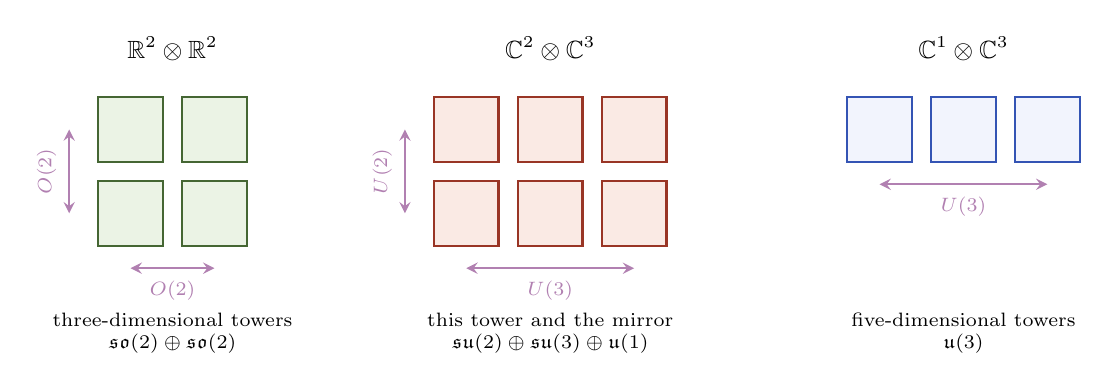
\begin{tikzpicture}[scale=0.82, >=stealth]
\begin{scope}[shift={(0,0)}]
\foreach \i in {0,1} {\foreach \j in {0,1} {\draw[OliveGreen!70!black, thick, fill=OliveGreen!8] (\j*1.3, -\i*1.3) rectangle ++(1.0,1.0);}}
\node[font=\small] at (1.15, 1.75) {$\R^{2} \otimes \R^{2}$};
\draw[<->, thick, Plum!80!black] (-0.45, 0.5) -- (-0.45, -0.8); \node[Plum!80!black, font=\scriptsize, rotate=90] at (-0.8, -0.15) {$O(2)$};
\draw[<->, thick, Plum!80!black] (0.5, -1.65) -- (1.8, -1.65); \node[Plum!80!black, font=\scriptsize] at (1.15, -2.0) {$O(2)$};
\node[font=\scriptsize, align=center] at (1.15, -2.65) {three-dimensional towers\\$\so(2) \oplus \so(2)$};
\end{scope}
\begin{scope}[shift={(5.2,0)}]
\foreach \i in {0,1} {\foreach \j in {0,1,2} {\draw[BrickRed!80!black, thick, fill=BrickRed!7] (\j*1.3, -\i*1.3) rectangle ++(1.0,1.0);}}
\node[font=\small] at (1.8, 1.75) {$\C^{2} \otimes \C^{3}$};
\draw[<->, thick, Plum!80!black] (-0.45, 0.5) -- (-0.45, -0.8); \node[Plum!80!black, font=\scriptsize, rotate=90] at (-0.8, -0.15) {$U(2)$};
\draw[<->, thick, Plum!80!black] (0.5, -1.65) -- (3.1, -1.65); \node[Plum!80!black, font=\scriptsize] at (1.8, -2.0) {$U(3)$};
\node[font=\scriptsize, align=center] at (1.8, -2.65) {this tower and the mirror\\$\su(2) \oplus \su(3) \oplus \uu(1)$};
\end{scope}
\begin{scope}[shift={(11.6,0)}]
\foreach \j in {0,1,2} {\draw[RoyalBlue!80!black, thick, fill=RoyalBlue!7] (\j*1.3, 0) rectangle ++(1.0,1.0);}
\node[font=\small] at (1.8, 1.75) {$\C^{1} \otimes \C^{3}$};
\draw[<->, thick, Plum!80!black] (0.5, -0.35) -- (3.1, -0.35); \node[Plum!80!black, font=\scriptsize] at (1.8, -0.7) {$U(3)$};
\node[font=\scriptsize, align=center] at (1.8, -2.65) {five-dimensional towers\\$\uu(3)$};
\end{scope}
\end{tikzpicture}
\caption{The minimal massive hierarchies: rows are constituents at mass onset, columns their ladder pairs. Two real constituents of two real pairs in three dimensions (orthogonal slot and pair groups, an abelian gauge algebra); two complex constituents of three pairs in four dimensions (T12's Standard-Model algebra); one constituent of three pairs in five dimensions (colour and one abelian charge). The automorphisms respecting both factors are the gauge algebras of Theorem \ref{thm:algebras}.}
\label{fig:grids}
\end{figure}

\begin{remark}[branches that break U, and what they give]\label{rem:branches}
Two transpositions reproduce this tower and break a clause of Premise \ref{prem:U}. (a) Counting the $r = 7$ constituent in the full Clifford module, where the central $\omega$ joins two real constituents into one complex element that is already massive (Theorem \ref{thm:onset}(i) for the two real parts), gives the hierarchy $\C^{1} \otimes \C^{2}$ and $\uu(2)$, with content a doublet of $Y = \tfrac{1}{2}$, a singlet of $Y = -1$ and a neutral singlet; it breaks U1, since $\omega$ is odd and does not act on the spin-irreducible ideal (Proposition \ref{prop:omega7}(ii)). (b) Building the five-dimensional third pair with an external $i$, which commutes with the quaternionic unit group, keeps that group as the slot group of the one constituent: the hierarchy is a quaternionic line tensor $\C^{3}$, with automorphisms $\su(2) \oplus \su(3) \oplus \uu(1)$ and global form $S(U(2) \times U(3))$, and vector-like content $(2,3)_{1/6}$, $(2,1)_{-1/2}$. It keeps U1 and U2 and breaks U3; it is T12's own practice of working in the complexification, carried to a tower whose field is $\HH$; and it is open at $r = 3$ and $r = 5$ on the same terms, so it does not separate them. Its $\su(2)$ acts on one constituent's quaternionic multiplicity, not on two constituents. Their arithmetic is in the supplementary scripts (\file{D3C}, \file{D5Q}; Section \ref{sec:verification}). Neither is a result of this paper.
\end{remark}

%=====================================================================================
\section{Content}\label{sec:content}

T12's lesson is that fermions are generators of the composite, not its states \cite[Rem.~5.2, Prop.~5.3]{ButlerT12}. The generators of a hierarchy $\F^{m} \otimes \F^{k}$ are its single slot-pair cells; Hypothesis (S) adds the constituent-level states.

\begin{proposition}[the three-dimensional content]\label{prop:content3}
In the towers $r = 1, 7$:
\begin{enumerate}
\item[(i)] The generators are the four cells of $\R^{2} \otimes \R^{2}$, of weights $(s, p) \in \{\pm 1\}^{2}$; as complex two-component fermions they are $A$, with $(q_{+}, q_{-}) = (1, 0)$, and $B$, with $(0, 1)$, and their conjugates. Each is charged under one factor only: the tower is two copies of single-flavour electrodynamics in $2+1$ dimensions, exchanged by the pair reflection $p \mapsto -p$.
\item[(ii)] Every weight of the exterior algebra of the cells has $s + p$ even; no state of the tensor state space has weight $(\pm 1, 0)$ or $(0, \pm 1)$.
\item[(iii)] Under (S) the constituent-level states have weight $(\pm 1, 0)$, off the lattice $s + p$ even: (S) and the global form of Theorem \ref{thm:algebras}(i) are incompatible. Of the directions the transport adds, the rung directions carry $(\pm 1, 0)$ and the pair directions $(0, \pm 1)$, and both are excluded; the one neutral direction (the leftover generator of the odd conformal algebra) is allowed, and its value is a bare mass. The tower has no charged Higgs analogue.
\item[(iv)] There is no chirality: the odd-dimensional modules carry no Lorentz-invariant grading \cite[Prop.~3.9]{ButlerT14}. Gauge-invariant Dirac masses exist for $A$ and $B$ without any condensate, and there is no baryon-like composite: every gauge-neutral state has zero net number of each cell.
\end{enumerate}
\end{proposition}

\begin{proof}
\textit{(i)}\enspace The cells are single-occupation states. The charges $q_{\pm} = (s \pm p)/2$ send
\[
(s, p) = (1, 1) \;\mapsto\; (q_{+}, q_{-}) = (1, 0), \qquad (1, -1) \;\mapsto\; (0, 1) \qquad \text{(F2)},
\]
and the pair reflection $p \mapsto -p$ exchanges them.

\pitem{(ii)} A product of cells adds weights, and each cell has $s + p \in \{-2, 0, 2\}$ (F1).

\pitem{(iii)} A constituent-level state occupies one slot mode and no pair mode, so its weight is $(\pm 1, 0)$, off the lattice $s + p$ even (Remark \ref{rem:S35}). The weights of the transported directions are computed in the supplementary script \file{D3R} (checks H5 to H9): rung directions $(\pm 1, 0)$, pair directions $(0, \pm 1)$, the leftover generator $(0,0)$.

\pitem{(iv)} This is the odd case of T14's Proposition 3.9 (Fact \ref{fact:towers}). A mass term $\bar{A}A$ has weight zero, and a neutral product of cells pairs each cell with its conjugate.
\end{proof}

\begin{remark}[the neutral row]\label{rem:neutralrow}
In a hierarchy $\C^{1} \otimes \C^{k}$ whose central generator acts by $k$ on the slot and $-1$ on each pair, the state with the slot and all $k$ pairs occupied has weight $k - k = 0$. The constituent-level generator of a one-constituent hierarchy is therefore neutral: the trace-free central generator of $\uu(1) \oplus \uu(k)$ on $\C^{1} \oplus \C^{k}$ is $(k\,i, -i\,1_{k})$ up to scale, and weights add. Arithmetic.
\end{remark}

\begin{proposition}[the five-dimensional content]\label{prop:content5}
In the towers $r = 3, 5$, under (S) the state space $\Lambda^{\bullet}(\C^{1} \oplus \C^{3})$ has sixteen states. With $Y = s - k/3$ ($s$ the slot occupation, $k$ the number of occupied pairs), the complement $(s,k) \mapsto (1-s, 3-k)$ negates $Y$ and conjugates colour, so the sixteen are eight species-states and their conjugates, four vector-like Dirac species:
\begin{center}\small
\begin{tabular}{@{}lccl@{}}
\toprule
species & colour & $Y$ & states $(s,k)$ \\
\midrule
$U$ & $3$ & $2/3$ & $(1,1)$, conjugate $(0,2)$ \\
$D$ & $3$ & $-1/3$ & $(0,1)$, conjugate $(1,2)$ \\
$E$ & $1$ & $-1$ & $(0,3)$, conjugate $(1,0)$ \\
$N$ & $1$ & $0$ & $(0,0)$, $(1,3)$ \\
\bottomrule
\end{tabular}
\end{center}
These are the electric charges of one of our generations with the weak doublet removed. Through the section $B \mapsto ((\det B)^{-1}, B)$ the centre of $U(3)$ acts on $(s,k)$ by $\lambda^{k - 3s} = \lambda^{-3Y}$, so $3Y$ is an integer with $3Y + k \equiv 0 \pmod 3$, $k$ being the triality: the lattice of $U(3)$, satisfied automatically; the neutral species $N$ is the empty state and the full row of Remark \ref{rem:neutralrow}. Without (S) the content is one Dirac colour triplet of $Y = 2/3$. There is no chirality and every species has a gauge-invariant bare mass.
\end{proposition}

\begin{proof}
The state space has
\[
\dim \Lambda^{\bullet}\C^{4} \;=\; \sum_{s=0}^{1}\sum_{k=0}^{3}\binom{3}{k} \;=\; 2 \cdot 8 \;=\; 16
\]
states, the $\binom{3}{k}$ states at pair number $k$ forming the $1, 3, \bar{3}, 1$ of $SU(3)$. The complement negates $Y$:
\[
Y(1 - s, 3 - k) \;=\; (1 - s) - \frac{3 - k}{3} \;=\; -\Bigl(s - \frac{k}{3}\Bigr) \;=\; -Y(s, k),
\]
and the remaining weights are arithmetic (F3, F4). The masses are as in Proposition \ref{prop:content3}(iv).
\end{proof}

\begin{remark}[why (S) fails in three dimensions and not in five]\label{rem:S35}
In both cases the slot-level states are charged under the kernel of the action on the hierarchy. In five dimensions the kernel is the common scalar $U(1)$, and the subgroup $S(U(1) \times U(3)) = \{((\det B)^{-1}, B)\}$ maps isomorphically onto the quotient $U(3)$: the exterior algebra of slot and pair modes is a representation of that section, as T12 uses $S(U(2) \times U(3))$ in four dimensions. In three dimensions the kernel $\{\pm(1,1)\}$ is discrete inside the torus $SO(2) \times SO(2)$, and no subgroup maps isomorphically onto the quotient, so the slot-level states are not representations of the global form. Under (S) the five-dimensional state space has a tenth abelian automorphism, the slot number, beyond the nine of $\uu(3)$; this paper takes it as a global symmetry, not gauged (a choice: T12 counts the corresponding extra generator in four dimensions and finds it anomaly-free, broken by the right-handed neutrino's Majorana mass \cite[Prop.~5.8]{ButlerT12}); here it is broken only by a mass term for $N$ off the pair unit's axis.
\end{remark}

\begin{proposition}[anomalies]\label{prop:anomaly}
\begin{enumerate}
\item[(i)] In the three-dimensional towers each $U(1)_{\pm}$ couples to exactly one unit-charge two-component fermion, which shifts its Chern-Simons level by $\tfrac{1}{2}\mathrm{sign}(m)$ (Fact \ref{fact:threeD}(i)); integrality of the effective level forces the bare levels into $\mathbb{Z} + \tfrac{1}{2}$. Parity is therefore broken by the gauge sector.
\item[(ii)] In the five-dimensional towers, in units $q' = 3Y$, the content of Proposition \ref{prop:content5} has $\sum q'^{3} = -6$ and $\sum q' = 0$ (with multiplicities), and the induced abelian cubic Chern-Simons coefficient, $\tfrac{1}{2}\sum \mathrm{sign}(m)\,q'^{3}$, is integral for every choice of mass signs, as Fact \ref{fact:fiveD} requires. The $SU(3)$ and mixed levels, which on $U(3)$ are tied to the abelian one, are not analysed here.
\end{enumerate}
\end{proposition}

\begin{proof}
\textit{(i)}\enspace With bare level $k$ and one unit-charge fermion of mass $m$, the effective level is
\[
k_{\mathrm{eff}} \;=\; k + \tfrac{1}{2}\,\mathrm{sign}(m) \;\in\; \mathbb{Z} \quad\Longrightarrow\quad k \in \mathbb{Z} + \tfrac{1}{2} \qquad \text{(G1, G2)},
\]
and no half-integer is zero, so a parity-odd Chern-Simons term is always present.

\pitem{(ii)} In units $q' = 3Y$ the species of Proposition \ref{prop:content5} carry $q' = 2, -1, -3, 0$ for $U, D, E, N$, with colour multiplicity $3$ for $U$ and $D$. So
\begin{align*}
\sum q'^{3} &= 3(2)^{3} + 3(-1)^{3} + (-3)^{3} + 0 = 24 - 3 - 27 = -6, \\
\sum q' &= 3(2) + 3(-1) + (-3) + 0 = 0 \qquad \text{(G3)}.
\end{align*}
In $\tfrac{1}{2}\sum \mathrm{sign}(m)\,q'^{3}$ the terms of $U$ and $N$ are the integers $\pm 12$ and $0$, and those of $D$ and $E$ are $\pm\tfrac{3}{2}$ and $\pm\tfrac{27}{2}$, whose sum is an integer for each choice of signs.
\end{proof}

%=====================================================================================
\section{The paired towers}\label{sec:paired}

T14's indifference premise P2 equates the data of the two members of each reversal pair, $\{2, 6\}$, $\{1, 7\}$ and $\{3, 5\}$ \cite[Prem.~2.2]{ButlerT14}. This section compares the members of the odd pairs as algebras.

\begin{proposition}[the residue-seven unit]\label{prop:omega7}
\begin{enumerate}
\item[(i)] Along the residue-seven tower ($\Cl(2,3)$, $\Cl(3,4)$, $\Cl(4,5)$, \ldots) the pseudoscalar is central and squares to $-1$ at every rung; along the residue-one tower ($\Cl(3,2)$, $\Cl(4,3)$, \ldots) it is central and squares to $+1$.
\item[(ii)] At $r = 7$ the pseudoscalar $\omega$ is odd: it carries the even ideal into the odd one, so it does not act on the constituent ideal, and the grade involution reverses it.
\item[(iii)] On the Clifford module $\Cl(\hatV)\hf = T \oplus \omega T$, left multiplication by $c + s\omega$ ($c^{2} + s^{2} = 1$) commutes with the whole Clifford action and carries $X + \omega Y$ to $(cX - sY) + \omega(sX + cY)$: on a pair of real constituents it is the slot rotation of Theorem \ref{thm:algebras}(i), here supplied by the algebra itself. Every cell carries charge $\pm 1$ under it. If the tower's action is built from operations that commute with the Clifford action, as T12's are, a Majorana-type mass (charge $2$) is then forbidden in the $r = 7$ tower whether or not the rotation is gauged; this last clause is at assembly level.
\end{enumerate}
\end{proposition}

\begin{proof}
\textit{(i)}\enspace By the formula of Section \ref{sec:setting}, $Q(\omega) = (-1)^{n(n-1)/2}(-1)^{q}$. Each rung adds $(1,1)$ to the signature, so $n$ rises by two and $q$ by one, and the first exponent changes by
\[
\frac{(n+2)(n+1)}{2} - \frac{n(n-1)}{2} \;=\; 2n + 1,
\]
which is odd. The two sign changes cancel, so $Q(\omega)$ is constant along each tower and equal to its value at the first rung:
\[
Q(\omega_{2,3}) = (-1)^{10}(-1)^{3} = -1, \qquad Q(\omega_{3,2}) = (-1)^{10}(-1)^{2} = +1.
\]
Every rung has odd dimension, so $\omega$ is central (H1, H2).

\pitem{(ii)} $\omega$ is a product of five vectors (H3), so it is odd, left multiplication by it exchanges the even and odd parts, and $\hat{\omega} = (-1)^{5}\omega = -\omega$.

\pitem{(iii)} $\omega$ is central with $\omega^{2} = -1$ (H4), so $c + s\omega$ commutes with the Clifford action, and for $X, Y \in T$
\[
(c + s\omega)(X + \omega Y) \;=\; cX + s\omega^{2}Y + \omega(sX + cY) \;=\; (cX - sY) + \omega(sX + cY).
\]
\end{proof}

\begin{corollary}[same kind of matter]\label{cor:samekind}
Under H2 and Premise \ref{prem:U} the two towers of each odd dimension have the same constituent field, the same mass onset, the same gauge algebra and the same content. They differ only as follows.
\begin{center}\small
\begin{tabular}{@{}p{3.6cm}p{4.9cm}p{4.9cm}@{}}
\toprule
 & $r = 1$ & $r = 7$ \\
\midrule
slot rotation & a rotation of two modules of the same type & the algebra's central unit, exact at every rung \\
slot reflection & internal & exists only fused with orientation reversal \\
module types & two ($\omega = \pm 1$) & one \\
number-violating masses & forbidden once the slot rotation is gauged (H2) & forbidden by the algebra's unit, gauged or not \\
\midrule
 & $r = 3$ & $r = 5$ \\
\midrule
the pair unit & $I_{7}$, fixed by the algebra & a point of $S^{2}$, not fixed \\
reversion-type invariant form & one, Hermitian for $I_{7}$ & none \\
module types & one & two \\
\bottomrule
\end{tabular}
\end{center}
\end{corollary}

\begin{proof}
The shared rows are Theorems \ref{thm:fields}, \ref{thm:onset}, \ref{thm:algebras} and Propositions \ref{prop:content3}, \ref{prop:content5}. The differing rows come from Proposition \ref{prop:omega7} and Theorem \ref{thm:unit}, except two that are computed in supplementary scripts: the slot-reflection row in \file{D3C} (Part I), and the invariant-form row in the referee script \file{CHECK\_ALG/check\_r3\_r5.py}.
\end{proof}

\begin{remark}[the $r = 5$ unit: datum or field]\label{rem:r5unit}
If the unit $u$ of Theorem \ref{thm:unit}(iii) is a constant of the tower, every choice gives an isomorphic tower and nothing observable distinguishes it from $r = 3$; this is how this tower treats its own unit, which the algebra fixes up to sign. If $u$ varies over spacetime, the tower carries a sigma model on $S^{2}$ with two massless five-dimensional scalars, which moves the radiation bound of Computation \ref{prop:fiveD}(iii) from $0.085$ to $0.084$. The series supplies no kinetic term for $u$; the first reading is this tower's.
\end{remark}

%=====================================================================================
\section{The mirror}\label{sec:mirror}

\begin{theorem}[the mirror as an algebra]\label{thm:mirror}
\begin{enumerate}
\item[(i)] The linear map $e_{K} \mapsto (-1)^{|K|/2}e_{K}$ on even basis blades is an algebra isomorphism from the even algebra of a signature onto the even algebra of the reversed signature (every $Q(e_{a})$ negated); in particular $\Cl^{0}(3,1) \cong \Cl^{0}(1,3)$ and $\Cl^{0}(4,2) \cong \Cl^{0}(2,4)$.
\item[(ii)] It carries the mirror's pseudoscalar $I_{4}'$ to $+I_{4}$ and its conformal pseudoscalar $I_{6}'$ to $-I_{6}$.
\item[(iii)] The full algebras differ: $\Cl(1,3)$ has quaternionic irreducible modules and $\Cl(3,1)$ real ones.
\end{enumerate}
\end{theorem}

\begin{proof}
\textit{(i) The product rule.}\enspace Write $Q$ for the squares of the first signature and $Q' = -Q$ for those of the second. For even blades $e_{K}$, $e_{L}$,
\[
e_{K}e_{L} \;=\; \sigma \prod_{c \in K \cap L}Q(e_{c})\;e_{K \triangle L},
\]
with $\sigma$ the reordering sign, which does not depend on the squares; the same holds in the second algebra with $Q'$ in place of $Q$.

\pstep{(i) The map respects it} Let $\varphi(e_{K}) = (-1)^{|K|/2}e_{K}$, and use $|K \triangle L| = |K| + |L| - 2|K \cap L|$ and $\prod_{c}Q'(e_{c}) = (-1)^{|K \cap L|}\prod_{c}Q(e_{c})$. Then
\begin{align*}
\varphi(e_{K}e_{L}) &= \sigma\prod_{c}Q(e_{c})\,(-1)^{|K \triangle L|/2}\,e_{K \triangle L}
= (-1)^{\frac{|K|+|L|}{2}}(-1)^{|K \cap L|}\,\sigma\prod_{c}Q(e_{c})\,e_{K \triangle L}, \\
\varphi(e_{K})\,\varphi(e_{L}) &= (-1)^{\frac{|K|+|L|}{2}}\,\sigma\prod_{c}Q'(e_{c})\,e_{K \triangle L}
= (-1)^{\frac{|K|+|L|}{2}}(-1)^{|K \cap L|}\,\sigma\prod_{c}Q(e_{c})\,e_{K \triangle L}.
\end{align*}
The two agree. The script checks every pair of basis blades in both cases (I1).

\pitem{(ii)} On the pseudoscalars,
\[
\varphi(I_{4}') = (-1)^{4/2}\,I_{4} = +I_{4}, \qquad \varphi(I_{6}') = (-1)^{6/2}\,I_{6} = -I_{6} \qquad \text{(I2)}.
\]

\pitem{(iii)} The commutants are $\HH$ and $\R$ (I3; Fact \ref{fact:clifford}).
\end{proof}

So the mirror's constituents are complex, as ours are (Theorem \ref{thm:fields}): its real (Majorana) ground spinors do not make them real. The isomorphism sends the mirror's field unit $I_{4}'$ to ours and its conformal unit $I_{6}'$ to minus ours. If each tower's constituent unit is taken to be its own oriented conformal pseudoscalar, the mirror's constituent unit and field unit therefore have the opposite relative sign to ours, and the mirror is the parity image of this tower. That reading is interpretive and depends on the identification of the transported plane, which with one sign reversed would flip the sign of $I_{6}'$'s image. Nothing gravitational distinguishes the two.

\begin{proposition}[the mirror's temperature and P2]\label{prop:P2}
T14 applies P2 along the reversal orbit to equate the ceiling coupling and the asymmetry per mode, both data of the descent \cite[Thm.~4.3(iv), (v)]{ButlerT14}. The energy the descent deposits per unit charge is a datum of the same kind, and P2 declares which of $2$, $6$ is visible to be indexical. Applied with the same reach, P2 gives $\xi = T'/T = 1$ and $\Delta\Neff = \tfrac{8}{7}(\tfrac{11}{4})^{4/3} + 3.044 = 7.45$ at recombination, excluded by a factor of about $25$. T14's mirror, cold from the gravitational floor upward \cite[Prop.~4.6, Prop.~A.2]{ButlerT14}, is therefore an exception to P2 that T14 neither states nor costs. Assembly level.
\end{proposition}

\begin{proof}
\textit{The reach of P2.}\enspace The equalities of T14's Theorem 4.3(iv), (v) rest on P2's clause that a difference between two continuous data of one reversal orbit is an uncaused distinction. T14's Proposition A.2 calls what the descent deposited ``a datum, not a computation''.

\pstep{The number} At $\xi = 1$ the mirror is a full Standard-Model copy at the photon temperature. Its energy density is that of a photon, worth $\tfrac{8}{7}(\tfrac{11}{4})^{4/3}$ neutrino species, plus three neutrinos:
\[
\Delta\Neff \;=\; \underbrace{\tfrac{8}{7}\bigl(\tfrac{11}{4}\bigr)^{4/3}}_{\text{mirror photon}} \;+\; \underbrace{3.044}_{\text{mirror neutrinos}} \;=\; 4.40 + 3.044 \;=\; 7.45 \qquad \text{(K2)}.
\]
\end{proof}

\begin{computation}[the mirror's composition]\label{comp:mirror}
Decimal. Supplementary scripts: the mirror's (folder \file{MIR}, checks D1, D2 and E0 to E7) and the cosmology check's (folder \file{CHECK\_COS}). T14 carries $\xi$ from the gravitational floor ($2.8$ to $3.2 \times 10^{-4}$ at the top of the ceiling range) to the $\Neff$ cap ($0.448$), with a hot-deposit estimate near $4 \times 10^{-3}$.
\begin{enumerate}
\item[(i)] At the floor the mirror is charge-dominated and degenerate from the moment it is seeded: the Fermi energy its deposited baryon number must carry exceeds the floor's thermal deposit by $49$ to $84$, and at its weak freeze-out the quark chemical potential is $18$ to $23$ times its temperature. Beta equilibrium persists into the hadron phase, and for a copied lepton number $L \leq 0$ (our tower's sphaleron value $L/B = -51/28$, or zero) the mirror ends $96$ to $100$ percent neutrons. Its endpoint is cold, dense, neutron-rich matter; the composition after decay and capture needs a dense-matter network and is not computed here.
\item[(ii)] Between $\xi \approx 3 \times 10^{-3}$ and $2 \times 10^{-2}$, an interval containing T14's hot-deposit estimate, the mirror is helium ($Y' = 0.94$ to $1.00$).
\item[(iii)] Above that interval the helium fraction falls ($Y' = 0.85$ at $\xi = 0.1$) and towards the cap the mirror is hydrogen-rich ($Y' = 0.58$ at $\xi = 0.448$).
\end{enumerate}
T14 does not print a mirror $\eta'$ at freeze-out; its floor value $19$ to $26$ is the late-time ratio, and the thermal up-down ratio T14 assumes there is inconsistent with its own $\eta' > 1$.
\end{computation}

\begin{figure}[ht]
\centering
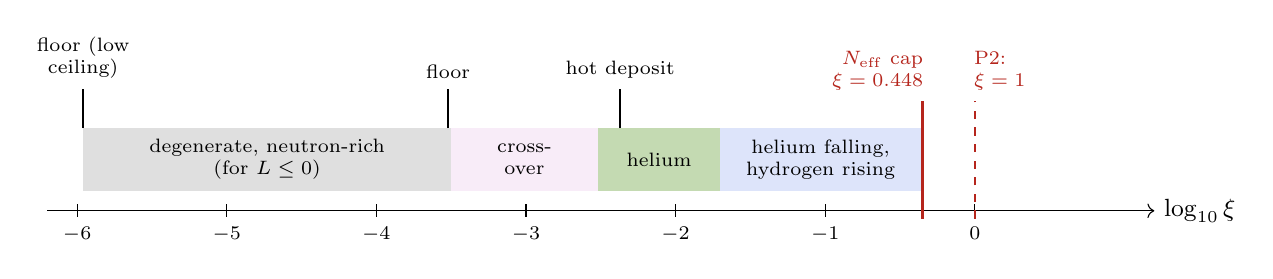
\begin{tikzpicture}[xscale=1.9, yscale=1]
\draw[->] (-0.2,0) -- (7.2,0) node[right, font=\small] {$\log_{10}\xi$};
\foreach \x/\l in {0/-6, 1/-5, 2/-4, 3/-3, 4/-2, 5/-1, 6/0} {\draw (\x,0.08) -- (\x,-0.08) node[below, font=\scriptsize] {$\l$};}
\fill[gray!25] (0.04,0.25) rectangle (2.5,1.05); \node[font=\scriptsize, align=center] at (1.27,0.65) {degenerate, neutron-rich\\(for $L \leq 0$)};
\fill[Plum!20] (2.5,0.25) rectangle (3.48,1.05); \node[font=\scriptsize, align=center] at (2.99,0.65) {cross-\\over};
\fill[OliveGreen!25] (3.48,0.25) rectangle (4.3,1.05); \node[font=\scriptsize, align=center] at (3.89,0.65) {helium};
\fill[RoyalBlue!18] (4.3,0.25) rectangle (5.65,1.05); \node[font=\scriptsize, align=center] at (4.97,0.65) {helium falling,\\hydrogen rising};
\draw[BrickRed, thick] (5.65,-0.1) -- (5.65,1.4) node[above left, font=\scriptsize, align=right, xshift=4pt] {$\Neff$ cap\\$\xi = 0.448$};
\draw[BrickRed, thick, dashed] (6,-0.1) -- (6,1.4) node[above right, font=\scriptsize, align=left, xshift=-4pt] {P2:\\$\xi = 1$};
\draw[black, thick] (2.48,1.05) -- (2.48,1.55) node[above, font=\scriptsize] {floor};
\draw[black, thick] (0.04,1.05) -- (0.04,1.55) node[above, font=\scriptsize, align=center] {floor (low\\ceiling)};
\draw[black, thick] (3.63,1.05) -- (3.63,1.55) node[above, font=\scriptsize] {hot deposit};
\end{tikzpicture}
\caption{The mirror's composition against its temperature ratio $\xi = T'/T$ (Computation \ref{comp:mirror}). T14 carries the whole interval from its gravitational floor to the $\Neff$ cap; P2 applied with T14's reach would put the mirror at $\xi = 1$, outside it.}
\label{fig:mirror}
\end{figure}

\begin{observation}[the mirror against the record]\label{obs:mirror}
On every branch the mirror recombines early (at a visible temperature of $0.04$ to $3$ keV) and is cold dark matter for the microwave background and large-scale structure, and in galaxies it is a collisional gas that cools by bremsstrahlung in a few gigayears, settles partly and forms stars. Against the Gaia thin-disk bounds \cite{Widmark2021} and Roux and Cline's limit $\Omega_{b'} \lesssim 0.8\,\Omega_{b}$, their bound at low mirror temperature \cite{RouxCline2020},, only the helium interval has room: there T14b's Galaxy models pass at the Sun only with helium-star feedback \cite[Obs.~9.1]{ButlerT14b}, and Roux and Cline's limit, which covers the whole helium interval, is exceeded by a factor $1.24$. Nothing in the construction lowers the mirror's share below $0.995$ or changes its microphysics without a further exception to P2: the copy is exact and the tension T14 records stands. Observation level, on imported galaxy modelling.
\end{observation}

%=====================================================================================
\section{From content to matter}\label{sec:matter}

This section uses imported physics (Facts \ref{fact:threeD} to \ref{fact:plasma}) and decimal estimates, labelled; every number is reproduced by Part K of the script or by the named supplementary check. Its decimal estimates take T14's particle model (Fact \ref{fact:rule}): the quanta's mass is the nucleon's and $d$ is this world's baryon spacing, $d_{b} \approx 0.98$ m. E alone fixes the mass density and leaves both the number of quanta and $d$ free, so a statement below that uses a number density or the value of $d$ is conditional on that model. The five-dimensional statements of Computation \ref{prop:fiveD}(i), (ii) and (iv) need only $LT \gg 1$; the radiation caps of (iii) scale with $LT$.

\begin{observation}[the three-dimensional phases]\label{prop:phases}
By Fact \ref{fact:threeD}, with the minimal bare level $|k| = \tfrac{1}{2}$ of Proposition \ref{prop:anomaly}(i), each factor is in one of two phases, set by whether the cell's mass sign is aligned with its bare level:
\begin{enumerate}
\item[(C)] effective level $0$: Polyakov-confining; the cells bind into neutral onia that annihilate at full strength into a lighter channel;
\item[(T)] effective level $\pm 1$: topologically massive, the photon gapped at $e^{2}/2\pi$; the unit-charge lines are transparent and the cells become effectively neutral and, on the standard signs, spin $0$ (interpretive).
\end{enumerate}
In phase (T) with $e^{2} \gg m$ the cells are stable by their gauge charges (at $r = 7$ also by the algebra's central unit, Proposition \ref{prop:omega7}), and contact processes scale as $(m/e^{2})^{2}$. Assembly level. T14's Proposition 6.2 states that every compact $U(1)$ in three dimensions confines \cite[Prop.~6.2]{ButlerT14}; with the forced half-integral level that holds in phase (C) only. Both phases close T14's radiation channel: nothing light remains in phase (T), and even two massless $2+1$ dimensional photons at the photon temperature would give $\Delta\Neff$ of about $4 \times 10^{-3}$ on sheets (supplementary \file{CHECK\_COS}).
\end{observation}

\begin{computation}[survival on sheets]\label{prop:sheetsurvival}
Decimal. On a sheet the comoving number per unit area and the expansion rate both fall as $a^{-2}$ in radiation domination, so two-dimensional s-wave annihilation with $\sigma_{1}v = 2P/m$ ($P$ the absorption probability per encounter) depletes a symmetric population logarithmically, $1/N_{f} = 1/N_{0} + (2P/m)\ln(a_{f}/a_{i})/(a^{2}H)$. At the particle model's density a symmetric sheet relic keeps $99$ percent of its number only for $P$ below $1$ to $2 \times 10^{-16}$, the range spanning the number of relativistic species; at $P = 1$ a fraction of order $10^{-14}$ survives ($1.2 \times 10^{-14}$ with the inputs here, K3; T14 gives about $3 \times 10^{-14}$ for the same estimate \cite[Sec.~7.7]{ButlerT14}). In phase (T) this needs $e^{2}/m$ above $7 \times 10^{7}$ to $9 \times 10^{7}$, which also makes the relic collisionless in clusters (threshold $5.9 \times 10^{6}$, from the in-sheet phase-shift bound $1.7 \times 10^{-7}$ of T14b's cluster computation \cite[Comp.~3.3, Prem.~2.12]{ButlerT14b}) (K4). Phase (C) fails the particle model's density by itself.
\end{computation}

\begin{computation}[the five-dimensional towers]\label{prop:fiveD}
Decimal, with Facts \ref{fact:fiveD} and \ref{fact:plasma}. With the fifth direction one $d$ deep and co-expanding (R3), and $d = d_{b}$ (the particle model; \cite[Prem.~7.4, Rem.~7.9, Rem.~7.14]{ButlerT14}):
\begin{enumerate}
\item[(i)] $LT$ runs from about $390$ (at $g_{s} = 106.75$) to $1170$ today: the Kaluza-Klein spacing is always below $T/120$, so the towers are five-dimensional at the visible temperature and at their matter's mass scale (K5); at T14's small dark temperatures the dark bath itself is only a few Kaluza-Klein levels deep.
\item[(ii)] Five-dimensional gauge theory is infrared free; reducing to four dimensions gives a confinement scale below $\pi/L$ by a factor smaller than $e^{-250}$ even at strong coupling (K7), and the $1/r^{2}$ potential binds nothing unless the theory is within a factor of about eight of strong coupling at the quark mass (supplementary \file{D5C}, H3; \cite{CLP2000}). There are no dark hadrons and no dark atoms.
\item[(iii)] With the Kaluza-Klein tower populated, $\Delta\Neff < 0.3$ needs $T_{D}/T_{\gamma} < 0.085$ for the nine vectors of $\uu(3)$ ($0.13$ for one photon), not the $0.46$ to $0.51$ of T14's zero-mode formula \cite[Prop.~6.3]{ButlerT14}; a sector decoupled at a GeV would give about $670$ (K6). T14's own temperature estimates meet the corrected bound by orders.
\item[(iv)] Two-body scattering is collisionless by geometry, $\sigma_{\mathrm{eff}}/m = \sigma_{5}/(Lm) < 10^{-8}\ \mathrm{cm^{2}\,g^{-1}}$ even for charged and coloured species (supplementary \file{D5C}, H9).
\item[(v)] With no boundary term in the series the gauge field's natural condition at the ends of the fifth direction keeps a four-dimensional zero mode, so beyond about a metre the charged species form a neutral dark plasma. The plasma-instability limits of Fact \ref{fact:plasma}, rescaled to a GeV, lie six to ten orders below the coupling a freeze-out relic needs and about two to five orders below a deposit at a natural five-dimensional coupling (supplementary \file{D5C}, checks I3 and I4, and \file{CHECK\_COS}). Whether such instabilities transfer bulk momentum in a merger is not established (Fact \ref{fact:plasma}): an exposure, not an exclusion.
\item[(vi)] If the neutral species $N$ (Proposition \ref{prop:content5}) carries the particle model's count as a deposit and the charged species annihilate at weak coupling, the tower carries no long-range charge and is collisionless whatever the zero modes do. Under Premise \ref{prem:U} this branch is open to both five-dimensional towers.
\end{enumerate}
The relic is a symmetric gas of free spin-$\tfrac{1}{2}$ dark quarks and leptons, or of $N$ alone. The lightest species is stable by fermion parity, the lightest quark and lepton by species numbers broken only at the rung scale.
\end{computation}

\begin{observation}[neither E nor the particle model has a mechanism in the odd towers]\label{prop:R1}
In this tower and the mirror a quantum's mass is a confinement scale, $m = c\Lambda$ \cite[Prop.~4.7]{ButlerT14}. In the three-dimensional towers the gauge algebra is abelian and the coupling dimensionful, so there is no dimensional transmutation and the cells' masses are bare parameters; the viable phase needs $m/e^{2}$ below $1.1$ to $1.5 \times 10^{-8}$, which nothing in the content protects (no chirality; parity broken by the forced Chern-Simons level). In the five-dimensional towers nothing confines (Computation \ref{prop:fiveD}(ii)) and the quanta are elementary with bare masses. The odd towers carry no asymmetry, so nothing fixes their number either (Observation \ref{prop:population}). So nothing in the content fixes the masses or the densities that E equates across towers, for about $81$ percent of the dark matter; still less does it supply the particle model's equal masses. T14 already concedes that nothing sets an odd tower's quanta's mass to ours \cite[Rem.~7.8, Sec.~8]{ButlerT14}. What this note adds is the reason, and one correction: T14's Section 8 reads the odd towers' quanta as composites of sectors whose confinement scales the series does not derive, whereas here they are elementary in five dimensions and unconfined in the viable three-dimensional phase. Assembly level.
\end{observation}

\begin{observation}[population]\label{prop:population}
The odd towers carry no asymmetry (Fact \ref{fact:towers}). Their matter is therefore symmetric, and the number of quanta that fills E's density must be either a count deposited by the descent and protected from annihilation by kinematics or weakness (Computations \ref{prop:sheetsurvival}, \ref{prop:fiveD}(vi)), or, in the five-dimensional towers, a weak-coupling freeze-out with the coupling tied to the deposit temperature. Neither is derived. Assembly level.
\end{observation}

%=====================================================================================
\section{The sterile towers}\label{sec:sterile}

\begin{proposition}[the sterile kinematics]\label{prop:sterile}
\begin{enumerate}
\item[(i)] In $\R^{2,2}$ the orthogonal complement of every non-null vector is nondegenerate and indefinite, so every vector, of either sign of $Q$, is a sum of two null vectors $v = (\tfrac{1}{2}v + w) + (\tfrac{1}{2}v - w)$ with $w \perp v$, $Q(w) = -Q(v)/4$; and the null cone minus the origin is connected, so it has no invariant future half.
\item[(ii)] In $\R^{4,0}$ (and $\R^{0,4}$) the only null vector is zero: there is no massless constituent, no time and no evolution.
\end{enumerate}
\end{proposition}

\begin{proof}
\textit{(i) Sums of null vectors.}\enspace For non-null $v$, $v^{\perp}$ is three-dimensional, of signature $(1,2)$ if $Q(v) > 0$ and $(2,1)$ if $Q(v) < 0$. Either way $Q$ is indefinite on it, so it takes the value $-Q(v)/4$ at some $w \perp v$, and then
\[
Q\bigl(\tfrac{1}{2}v \pm w\bigr) \;=\; \tfrac{1}{4}Q(v) + Q(w) \;=\; \tfrac{1}{4}Q(v) - \tfrac{1}{4}Q(v) \;=\; 0
\]
(J1, which also checks nondegeneracy and indefiniteness on random vectors, and J2, which exhibits sums of both signs).

\pstep{(i) The cone is connected} In coordinates $(t_{1}, t_{2}; x_{1}, x_{2})$ with $Q = t_{1}^{2} + t_{2}^{2} - x_{1}^{2} - x_{2}^{2}$, the null cone minus the origin is
\[
\bigl\{\, |t| = |x| > 0 \,\bigr\} \;\cong\; S^{1} \times S^{1} \times \R_{>0},
\]
which is connected. In signature $(1,3)$ the same set has the two components $t_{0} > 0$ and $t_{0} < 0$. T16 proves the corresponding statement for the timelike sets \cite[Lem.~4.4]{ButlerT16}.

\pitem{(ii)} $Q$ is a sum of four squares, so $Q(v) = 0$ only at $v = 0$ (J3).
\end{proof}

\begin{remark}[the Kleinian algebra]\label{rem:kleinian}
At $r = 0$ the constituent field is $\R$ (Theorem \ref{thm:fields}), and $\Cl^{0}(2,2) \cong \Mat_{2}(\R) \oplus \Mat_{2}(\R)$ has two inequivalent spinor ideals. There is no time direction, so no adjoint and no norm clause: a momentum bilinear in one element of each ideal is preserved by acting with $U$ on the elements of the first ideal and $U^{-T}$ on those of the second, for every $U \in GL(n,\R)$ (supplementary \file{STE}, checks C4, C5). Under H2 with this slot group the gauge algebra is the split form $\sll(2,\R) \oplus \sll(3,\R) \oplus \gl(1,\R)$, of dimension $12$, whose simple factors have indefinite Killing forms, signatures $(2,1)$ and $(5,3)$ (E5): there is no positive gauge-kinetic energy. T14's ``Kleinian copy of the Standard Model'' \cite[Cor.~3.11]{ButlerT14} needs a compact weak factor, which does not preserve that bilinear. Assembly level.
\end{remark}

Both sterile towers are empty under T14's Premise P3, which is what the unit-ball rule's agreement with the observed ratio assumes: a populated $r = 0$ at share one would move the total to $6.36$, fifteen standard deviations from the observed $5.364 \pm 0.065$ \cite{Planck2018}.

%=====================================================================================
\section{The dark sector as built, against the data}\label{sec:data}

\begin{observation}[the towers as built]\label{obs:data}
\begin{center}\small
\begin{tabular}{@{}p{3.6cm}p{10.2cm}@{}}
\toprule
test & status \\
\midrule
$\Delta\Neff < 0.3$ & met on every branch except a hot mirror ($\xi = 1$, $7.45$) and a five-dimensional sector decoupled at a GeV (about $670$) \\
cluster mergers & passes T14b's mass-to-light test only if the mirror is the only colliding component, and even then the subcluster's own mass falls by more than the $23$ percent bound (Fact \ref{fact:sims}); that needs both three-dimensional towers in phase (T) at strong coupling with an unprotected light mass, and both five-dimensional towers collisionless (neutral-$N$ deposit, couplings weak near the unification scale, or ends the series does not supply). With zero modes and charged relics in both five-dimensional towers the colliding fraction would be $50.2$ percent, the fraction of T14b's failing mixed-count runs; with one, $34.4$ percent, above the $31.6$ percent run that already loses about half the subcluster's central mass. The extrapolation from fluids to a plasma is itself unproved \\
mirror bounds & marginal at best, in the helium interval with helium-star feedback, still $1.24$ above Roux and Cline; the helium interval itself needs an exception to P2 \\
E and the particle model & no mechanism in the odd towers, whose quanta have bare masses (Observation \ref{prop:R1}); equal masses hold only for the mirror \\
\bottomrule
\end{tabular}
\end{center}
No configuration of the five towers as built is compatible with every test at face value. The least exposed configuration needs four choices the series does not make (a P2 exception for the mirror's temperature, boosted mirror feedback, strong coupling with an unprotected light mass in the three-dimensional towers, and collisionless five-dimensional relics), and even with them it stays marginal, $1.24$ above Roux and Cline's limit. Observation level.
\end{observation}

%=====================================================================================
\section{What this note depends on, and what would refute it}\label{sec:refute}

\emph{Proved here, at proof level} (the two mass laws of Theorem \ref{thm:onset} by exact symbolic verification)\emph{:} Theorem \ref{thm:fields}, Lemma \ref{lem:norm}, Theorems \ref{thm:onset}, \ref{thm:ladder}, \ref{thm:unit} and \ref{thm:mirror}, Proposition \ref{prop:pairs}, Proposition \ref{prop:omega7}(i) to (iii) up to its last clause, Proposition \ref{prop:sterile}, and the algebra in Theorem \ref{thm:algebras} and Propositions \ref{prop:content3}, \ref{prop:content5}, \ref{prop:anomaly}.

\emph{Assembly, under named premises:} that the algebras of Theorem \ref{thm:algebras} are gauge algebras (H2), that a constituent's momentum is $j$ of its spinor part off dimension four (H1), the constituent-level content (S), the transposition rule (U), including the compactness of the pair group (U2), which is assumed and not derived, and Proposition \ref{prop:P2}, Observations \ref{prop:phases}, \ref{prop:R1}, \ref{prop:population}, Remark \ref{rem:kleinian}.

\emph{Decimal:} Computations \ref{comp:mirror}, \ref{prop:sheetsurvival}, \ref{prop:fiveD}, Observation \ref{obs:data}.

\emph{Interpretive:} the mirror as parity image; the spin $0$ of the dressed three-dimensional cells.

\emph{What would refute the constructions.} A spin-irreducible constituent ideal whose spin commutant differs from Theorem \ref{thm:fields}'s; a nonzero element of $S$ in dimension three or four with $\rev{\psi}\psi \neq 0$; an element of $\HH$ outside $\mathrm{span}\{1, I_{7}\}$ at $r = 3$ commuting with the $I_{7}$-built pair algebra. Each is a finite computation the script performs.

\emph{What would refute the physics.} A thin dark disk or bulge component excluding a mirror of $0.995\,\Omega_{b}$ in the helium interval with helium-star feedback refutes T14's mirror; a demonstration that dark plasma instabilities transfer bulk momentum in cluster mergers, with gauge zero modes in the five-dimensional towers, refutes the composition unless their relic is the neutral species; a measured $\Delta\Neff$ excess attributable to a dark sector would place a five-dimensional tower above $0.085$ of the photon temperature, outside T14's estimates.

\emph{Successor problems.} (1) Whether the cold mirror is a stated exception to P2, and where in T14's interval $\xi$ lies. (2) A footing for E's common length and equal mass per ball in the odd towers, where neither E nor the particle model has a mechanism; and, for T14, its Section 8's reading of the odd towers' quanta as confined composites, which Observation \ref{prop:R1} contradicts. (3) The boundary data of the five-dimensional towers' fifth direction (zero modes or not) and their population mechanism. (4) The three-dimensional phase and coupling. (5) Hypothesis (S) off dimension four, the same missing theorem as in this tower. (6) The family count in the odd towers, where the maximal-composite bound of T13 \cite[Conj.~3.1]{ButlerT13} does not transpose. (7) The $r = 5$ unit: datum or field. (8) Whether the five-dimensional pair unit is internal (U3) or external, which decides between $\uu(3)$ and the Standard-Model algebra in both towers. (9) The $SU(3)$ and mixed Chern-Simons levels of the five-dimensional content.

%=====================================================================================
\section{Position in the series}\label{sec:position}

This paper is T14c of the series, a companion to the dark-matter paper T14 \cite{ButlerT14}, downstream of its Theorem 3.4 (types by residue), Proposition 4.1 (superselection), Theorem 4.3 (the mirror copy), Theorem 3.10 (no orientation bit in odd dimension) and its unit-ball rule on Premises E and R3 (Section 7 of T14 Version 2.1). It runs the construction of the Standard-Model paper T12 \cite{ButlerT12} in each tower, using the mass formula of the mass paper T11 \cite{ButlerT11}, the rungs and canonical relations of the tower paper T3 \cite{ButlerT3}, and, for comparison only, the families of T13 \cite{ButlerT13} and the neutrino sector of T15 \cite{ButlerT15}. Its physical tests take the simulations of the companion note T14b \cite{ButlerT14b} as given; the companion note T14a \cite{ButlerT14a} is upstream of nothing here. The null-cone statement for signature $(2,2)$ is proved here (Proposition \ref{prop:sterile}); the foundations paper T16 proves the corresponding statement for the timelike sets \cite{ButlerT16}. The capstone T17 \cite{ButlerT17} records T14's predictions; Section \ref{sec:refute} lists what this note adds to them.

%=====================================================================================
\section{Machine verification}\label{sec:verification}

The script \file{verify\_T14c.py} \cite{ButlerVerifyT14c} imports the series library \file{GA.py} and checks the computational statements of Sections 3 to 10 in exact arithmetic: rational numbers, and a small polynomial ring over $\mathbb{Q}$ in which the identities of Lemma \ref{lem:norm} and Theorems \ref{thm:onset} and \ref{thm:ladder} are verified as polynomial identities in the spinors' coordinates rather than on samples. Part K alone is decimal and labelled. Without the supplementary scripts it runs $56$ checks, all passing:

\begin{center}\small
\begin{tabular}{@{}lll@{}}
\toprule
Part & statements & checks \\
\midrule
A & Theorem \ref{thm:fields} & A1 to A5 \\
B & Lemma \ref{lem:norm}, Theorem \ref{thm:onset} & B0 to B7 \\
C & Theorem \ref{thm:ladder} & C1, C2 \\
D & Proposition \ref{prop:pairs}, Theorem \ref{thm:unit} & D1a, D1b, D2 to D12 \\
E & Theorem \ref{thm:algebras}, Remark \ref{rem:kleinian} & E1 to E5 \\
F & Propositions \ref{prop:content3}, \ref{prop:content5} & F1 to F4 \\
G & Proposition \ref{prop:anomaly} & G1, G2 \\
H & Proposition \ref{prop:omega7} & H1 to H4 \\
I & Theorem \ref{thm:mirror} & I1 to I3 \\
J & Proposition \ref{prop:sterile} & J1 to J3 \\
K & Proposition \ref{prop:P2}, Computations \ref{prop:sheetsurvival}, \ref{prop:fiveD}; Fact \ref{fact:rule} (decimal) & K1 to K7 \\
\bottomrule
\end{tabular}
\end{center}

Part L runs the supplementary scripts, which are deposited with the paper in its folder \file{T14c\_supplement}: the derivation scripts \file{MIR}, \file{D3R}, \file{D3C}, \file{D5C}, \file{D5Q}, \file{STE} (one per tower: $24$, $61$, $78$, $86$, $106$ and $68$ checks) and two independent checks, \file{CHECK\_ALG} ($50$ exact checks) and \file{CHECK\_COS} (decimal, ten checks on the numbers this paper cites), and requires each to be present and to run clean, twelve further checks ($68$ in all). The script needs \texttt{scipy} for Part K and \file{CHECK\_COS}, and takes about two and a half minutes. The supplementary scripts' docstrings refer to working notes of the run that produced them; those notes are not part of the deposit, and nothing here relies on them. The paper cites them for the decimal composition of the mirror (Computation \ref{comp:mirror}), the five-dimensional binding, scattering and plasma estimates (Computation \ref{prop:fiveD}), the invariant forms of Corollary \ref{cor:samekind}, the branches of Remark \ref{rem:branches}, the Kleinian ladder of Remark \ref{rem:kleinian}, the transported weights of Proposition \ref{prop:content3}(iii) and the sheet radiation of Observation \ref{prop:phases}. What no script checks: the statement after Theorem \ref{thm:algebras} about the mirror (T14's), the imported physics (Redlich's shift, Polyakov, topological mass, flux attachment, five-dimensional Chern-Simons quantisation, plasma instabilities) and the galaxy modelling of T14b.

\begin{thebibliography}{99}

\bibitem{ButlerT3}
L.~Butler,
\emph{The Tower and the CAR Limit: Iterated Transport, the Frozen Clock, and Second Quantisation},
Transport Papers T3 (2026).

\bibitem{ButlerT9}
L.~Butler,
\emph{The Twistor Correspondence: Ascended Spinors, Incidence, and the Palatial Bridge},
Transport Papers T9 (2026).

\bibitem{ButlerT11}
L.~Butler,
\emph{The Origin of Mass: The Weight Dictionary and the Exact Join},
Transport Papers T11 (2026).

\bibitem{ButlerT12}
L.~Butler,
\emph{The Standard Model from the Minimal Massive Composite},
Transport Papers T12 (2026).

\bibitem{ButlerT13}
L.~Butler,
\emph{Quark and Lepton Families: Condensation, Democracy, and the Koide Relation},
Transport Papers T13 (2026).

\bibitem{ButlerT14}
L.~Butler,
\emph{Dark Matter and the Arrow of Time: The Dark Towers},
Transport Papers T14, Version 2.1 (2026), doi:\href{https://doi.org/10.5281/zenodo.22722953}{10.5281/zenodo.22722953}.

\bibitem{ButlerT14a}
L.~Butler,
\emph{One Dimension at a Time: The Odd Extensions of the Oriented Towers},
Transport Papers T14a (2026).

\bibitem{ButlerT14b}
L.~Butler,
\emph{Simulating the Dark Towers: Methods, Assumptions and Tests of the Unit-Ball Composition},
Transport Papers T14b (2026), deposited with its simulation code, run outputs and films.

\bibitem{ButlerT15}
L.~Butler,
\emph{Neutrino Masses: The Empty Twistor, the Seesaw Scale, and the Bet at the Floor},
Transport Papers T15 (2026).

\bibitem{ButlerT16}
L.~Butler,
\emph{Quantum Mechanics and General Relativity from One Relation: The Two Shadows and the Laboratory},
Transport Papers T16 (2026).

\bibitem{ButlerT17}
L.~Butler,
\emph{The Transport Programme: Method, Status, and the Falsifiable Ledger},
Transport Papers T17 (2026).

\bibitem{Chevalley1954}
C.~Chevalley,
\emph{The Algebraic Theory of Spinors},
Columbia University Press (1954).

\bibitem{Lounesto2001}
P.~Lounesto,
\emph{Clifford Algebras and Spinors}, 2nd ed.,
Cambridge University Press (2001).

\bibitem{Porteous1995}
I.~R.~Porteous,
\emph{Clifford Algebras and the Classical Groups},
Cambridge University Press (1995).

\bibitem{LawsonMichelsohn1989}
H.~B.~Lawson and M.-L.~Michelsohn,
\emph{Spin Geometry},
Princeton University Press (1989).

\bibitem{Hestenes1966}
D.~Hestenes,
\emph{Space-Time Algebra},
Gordon and Breach (1966); 2nd ed., Birkh\"auser (2015).

\bibitem{DoranLasenby2003}
C.~Doran and A.~Lasenby,
\emph{Geometric Algebra for Physicists},
Cambridge University Press (2003).

\bibitem{FootMirror2004}
R.~Foot,
\emph{Mirror matter-type dark matter},
Int. J. Mod. Phys. D \textbf{13} (2004), 2161--2192.

\bibitem{RouxCline2020}
J.-S.~Roux and J.~M.~Cline,
\emph{Constraining galactic structures of mirror dark matter},
Phys. Rev. D \textbf{102} (2020), 063518; arXiv:2001.11504.

\bibitem{Widmark2021}
A.~Widmark, C.~F.~P.~Laporte, P.~F.~de Salas, and G.~Monari,
\emph{Weighing the Galactic disk using phase-space spirals. II. Most stringent constraints on a thin dark disk using Gaia EDR3},
Astron. Astrophys. \textbf{653} (2021), A86.

\bibitem{Redlich1984}
A.~N.~Redlich,
\emph{Parity violation and gauge noninvariance of the effective gauge field action in three dimensions},
Phys. Rev. D \textbf{29} (1984), 2366--2374.

\bibitem{DJT1982}
S.~Deser, R.~Jackiw, and S.~Templeton,
\emph{Topologically massive gauge theories},
Ann. Phys. \textbf{140} (1982), 372--411.

\bibitem{AHPS1989}
I.~Affleck, J.~Harvey, L.~Palla, and G.~Semenoff,
\emph{The Chern-Simons term versus the monopole},
Nucl. Phys. B \textbf{328} (1989), 575--584.

\bibitem{Wilczek1982}
F.~Wilczek,
\emph{Quantum mechanics of fractional-spin particles},
Phys. Rev. Lett. \textbf{49} (1982), 957--959.

\bibitem{Polyakov1977}
A.~M.~Polyakov,
\emph{Quark confinement and topology of gauge theories},
Nucl. Phys. B \textbf{120} (1977), 429--458.

\bibitem{NiemiSemenoff1983}
A.~J.~Niemi and G.~W.~Semenoff,
Axial-anomaly-induced fermion fractionization and effective gauge-theory actions in odd-dimensional space-times,
\emph{Phys.~Rev.~Lett.} \textbf{51} (1983), 2077--2080.

\bibitem{IMS1997}
K.~Intriligator, D.~R.~Morrison, and N.~Seiberg,
\emph{Five-dimensional supersymmetric gauge theories and degenerations of Calabi-Yau spaces},
Nucl. Phys. B \textbf{497} (1997), 56--100.

\bibitem{CLP2000}
Z.~Chacko, M.~A.~Luty, and E.~Ponton,
\emph{Massive higher-dimensional gauge fields as messengers of supersymmetry breaking},
JHEP \textbf{07} (2000), 036.

\bibitem{SSS2024}
K.~M.~Schoeffler, N.~Shukla, and L.~O.~Silva,
\emph{Can plasma physics establish a significant bound on long-range dark matter interactions?},
arXiv:2411.15981 (2024).

\bibitem{PIC2024}
W.~DeRocco and P.~Giffin,
\emph{Dark plasmas in the nonlinear regime: constraints from particle-in-cell simulations},
arXiv:2411.11958 (2024).

\bibitem{Lasenby2020}
R.~Lasenby,
\emph{Long range dark matter self-interactions and plasma instabilities},
JCAP \textbf{11} (2020), 034; arXiv:2007.00667.

\bibitem{Planck2018}
N.~Aghanim et al. (Planck Collaboration),
\emph{Planck 2018 results. VI. Cosmological parameters},
Astron. Astrophys. \textbf{641} (2020), A6.

\bibitem{ButlerVerifyT14c}
L.~Butler,
\emph{verify\_T14c.py: machine verification for ``The Matter in the Dark Towers''},
Python script, deposited with this paper alongside the shared library GA.py and the supplementary scripts in T14c\_supplement (2026).

\end{thebibliography}

\end{document}
